\chapter{同调代数}

\section{线性代数的补充}

在本节中，字母 A 表示一个环。除非另有明确说明，所考虑的所有模均为左模，所有理想均为左理想。

这些定义和结果适用于右模，只需将它们视为相反环上的左模即可。

如果 M 是一个 A-模，并且如果 \(a \in A\) ，我们用 \(a_{M}\) 表示 M 的位似 \(x \mapsto ax\) 。因此我们有 \(1_{M} = Id_{M}\) （M 的恒等映射）；当不会产生混淆时，有时简写为 1 来代替 \(1_{M}\) .

最后，我们用 0 表示一个化为其单位元的 A-模，该模一经选定便固定下来（参见 II，第 8 页）。

\subsection{交换图}

设，例如，B、C、D、E、F 为五个集合，并设 \(f\) 是从 E 到 F 的映射， \(g\) 是从 B 到 C 的映射， \(h\) 是从 D 到 E 的映射， \(u\) 是从 B 到 D 的映射，且 \(v\) 是从C到E的一个映射。为了概括这类情形，人们常借助图表；例如，前述情形可用下图（E，II，第14页）来概括：

\[
\begin{array}{c} \mathrm{B} \xrightarrow {g} \mathrm{C} \\ u \Big \downarrow \\ \mathrm{D} \xrightarrow [ h ]{} \mathrm{E} \xrightarrow [ f ]{} \mathrm{F}. \end{array}\tag{1}
\]

在这样的图中，符号组 E \(\xrightarrow{f}\) F 示意了 f 是从 E 到 F 的映射这一事实。当对 f 不存在歧义时，可省略字母 f，直接写作 E \(\rightarrow\) F.

当B、C、D、E、F是群（相应地，A-模）且f、g、h、u、v是群（相应地，A-模）的同态时，为简洁起见，称图(1)为群（相应地，A-模）的图。

原则上，图不是数学对象，而仅仅是一个图形，旨在便于阅读证明。在实践中，人们常将图用作缩写符号，以避免逐一命名所有要考虑的集合和映射；因此，人们说“考虑图(1)”，而不是说：“设B、C、D、E、F为五个集合\ldots{} 且v为从C到E的映射”；例如参见第2节命题1的陈述。

例如，考虑下面的图表：

\[
\begin{array}{c} \mathrm{B} \xrightarrow {f} \mathrm{C} \xrightarrow {g} \mathrm{D} \xrightarrow {h} \mathrm{E} \\ b \Big \downarrow \qquad \qquad c \Big \downarrow \qquad \qquad d \Big \downarrow \qquad e \Big \downarrow \\ \mathrm{B} ^ {\prime} \xrightarrow {f ^ {\prime}} \mathrm{C} ^ {\prime} \xrightarrow {g ^ {\prime}} \mathrm{D} ^ {\prime} \xrightarrow {h ^ {\prime}} \mathrm{E} ^ {\prime}. \end{array}\tag{2}
\]

对于由图中若干段按箭头所示方向经过的线段组成的每条路径，都对应一个从第一段起点所表示集合到末段终点所表示集合的映射，即所经过各段对应映射的复合。对于图中的每个顶点，例如C，约定存在一条仅由C构成的路径，并约定与之对应恒等映射 1 \(_{C}\) .

在（2）中，例如，有三条从B出发、终止于D'的路径；相应的映射为 \(d \circ g \circ f\) , \(g' \circ c \circ f\) 和 \(g' \circ f' \circ b\) 。我们说一个图表是交换的，如果对于图表中具有相同起点和相同终点的每一对路径，对应的两个映射相等；特别地，如果一条路径的终点与其起点重合，则对应的映射必须是恒等映射。

为使图（2）可交换，其充要条件是以下关系式

\[
f ^ {\prime} \circ b = c \circ f, \qquad g ^ {\prime} \circ c = d \circ g, \qquad h ^ {\prime} \circ d = e \circ h;\tag{3}
\]

保持；换言之，从（2）中提取的三个方形图可交换是必要且充分的。事实上，关系式（3）蕴含 \(d \circ g \circ f = g' \circ c \circ f\) 因为 \(d \circ g = g' \circ c\) ，以及 \(g' \circ c \circ f = g' \circ f' \circ b\) ，因为 \(c \circ f = f' \circ b\) 因此，从B出发并以D'结束的三条路径给出相同的映射。类似地可以验证，从B出发并以E'结束的四条路径（分别地，从C出发并以E'结束的三条路径）给出相同的映射。关系式(3)意味着从B（分别地，C、D）出发并以C'（分别地，D'、E'）结束的两条路径给出相同的映射。(2)中所有其他顶点对至多由一条路径连接，因此图(2)确实是可交换的。

在下文中，我们将把对其他类型图表进行类似结果的表述与验证这一任务留给读者。

\subsection{蛇形图}

命题 1. --- 考虑一个 A-模的交换图

\[
\begin{array}{c} \mathrm{M} \xrightarrow {u} \mathrm{N} \xrightarrow {v} \mathrm{P} \\ f \Big \downarrow \qquad \qquad \qquad g \Big \downarrow \qquad \qquad \qquad h \Big \downarrow \\ \mathrm{M} ^ {\prime} \xrightarrow {u ^ {\prime}} \mathrm{N} ^ {\prime} \xrightarrow {v ^ {\prime}} \mathrm{P} ^ {\prime}. \end{array}\tag{4}
\]

假设 (4) 的两行是正合的。则：

\begin{enumerate}
\def\labelenumi{(\roman{enumi})}
\tightlist
\item
  若 h 是单射，我们有
\end{enumerate}

\[
\operatorname{Im} (g) \cap \operatorname{Im} \left(u ^ {\prime}\right) = \operatorname{Im} \left(u ^ {\prime} \circ f\right) = \operatorname{Im} (g \circ u).\tag{5}
\]

\begin{enumerate}
\def\labelenumi{(\roman{enumi})}
\setcounter{enumi}{1}
\tightlist
\item
  若 f 是满射，我们有
\end{enumerate}

\[
\operatorname{Ker} (g) + \operatorname{Im} (u) = \operatorname{Ker} \left(v ^ {\prime} \circ g\right) = \operatorname{Ker} (h \circ v).\tag{6}
\]

让我们证明 (i)。显然我们有

\[
\operatorname{Im} \left(u ^ {\prime} \circ f\right) = \operatorname{Im} (g \circ u) \subset \operatorname{Im} (g) \cap \operatorname{Im} \left(u ^ {\prime}\right).
\]

反之，设 \(y' \in \operatorname{Im}(g) \cap \operatorname{Im}(u')\) 。存在 \(y \in \mathbf{N}\) 使得 \(y' = g(y)\) 。由于 \(v' \circ u' = 0\) ，我们有 \(0 = v'(y') = v'(g(y)) = h(v(y))\) ，从而 \(v(y) = 0\) ，因为 \(h\) 是单射。由于 \((u, v)\) 是正合序列，存在 \(x \in \mathbf{M}\) 使得 \(y = u(x)\) ，从而 \(y' = g(u(x))\) .

让我们证明 (ii)。由于 \(v \circ u = 0\) 且 \(v' \circ u' = 0\) ，显然

\[
\operatorname{Ker} (g) + \operatorname{Im} (u) \subset \operatorname{Ker} \left(v ^ {\prime} \circ g\right) = \operatorname{Ker} (h \circ v).
\]

反之，设 \(y \in \operatorname{Ker}(v' \circ g)\) 。然后 \(g(y) \in \operatorname{Ker}(v')\) ，并且存在 \(x' \in M'\) 使得 \(u'(x') = g(y)\) 由于序列 \((u', v')\) 是正合的。由于 \(f\) 是满射的，存在 \(x \in M\) 使得 \(f(x) = x'\) ，从而 \(g(y) = u'(f(x)) = g(u(x))\) ；由此我们得出结论 \(y - u(x) \in \operatorname{Ker}(g)\) ，这就完成了证明。

引理1. —— 考虑一个A-模的交换图

\[
\begin{array}{c} \mathbf {M} \xrightarrow {\quad u \quad} \mathbf {N} \\ f \Big \downarrow \qquad \qquad \qquad \qquad \qquad \qquad \qquad \qquad g \Big \downarrow \\ \mathbf {M} ^ {\prime} \xrightarrow {\quad u ^ {\prime} \quad} \mathbf {N} ^ {\prime}. \end{array}\tag{7}
\]

那么存在唯一的同态 \(u_1: \text{Ker}(f) \to \text{Ker}(g)\) 和唯一的同态 \(u_2: \text{Coker}(f) \to \text{Coker}(g)\) ，使得以下图表

\[
\begin{array}{c} \operatorname{Ker} (f) \xrightarrow {u _ {1}} \operatorname{Ker} (g) \\ i \Biggl \downarrow \\ \mathrm{M} \xrightarrow [ u ]{} \mathrm{N} \end{array}\tag{8}
\]

和

\begin{enumerate}
\def\labelenumi{(\arabic{enumi})}
\setcounter{enumi}{8}
\tightlist
\item
\end{enumerate}

\pandocbounded{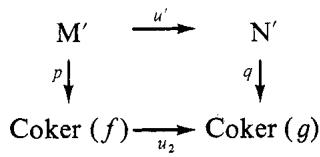
\includegraphics[keepaspectratio]{images/part001_11db974a.jpg}}

设它们是交换的，其中i和j表示典范单射，p和q表示典范满射。

事实上，若 \(x \in \operatorname{Ker}(f)\) ，我们有 \(f(x) = 0\) 和 \(g(u(x)) = u'(f(x)) = 0\) ，因此 \(u(x) \in \operatorname{Ker}(g)\) ，于是 \(u_1\) 的存在性与唯一性立即得出。同样地，我们有

\[
u ^ {\prime} (f (\mathbf {M})) = g (u (\mathbf {M})) \subset g (\mathbf {N}),
\]

因此 \(u'\) 通过取商给出一个同态

\[
u _ {2}: \operatorname{Coker} (f) \rightarrow \operatorname{Coker} (g),
\]

这是使（9）可交换的唯一同态。

现在从A-模的交换图（4）出发；根据引理1，它对应一个交换图

\[
\begin{array}{c c c c c} \operatorname{Ker} (f) \xrightarrow {u _ {1}} & \operatorname{Ker} (g) \xrightarrow {v _ {1}} & \operatorname{Ker} (h) \\ i \Big \downarrow & j \Big \downarrow & k \Big \downarrow \\ \mathbf {M} & u & \mathbf {N} & v & \mathbf {P} \\ f \Big \downarrow & g \Big \downarrow & h \Big \downarrow \\ \mathbf {M} ^ {\prime} & u ^ {\prime} & \mathbf {N} ^ {\prime} & v ^ {\prime} & \mathbf {P} ^ {\prime} \\ p \Big \downarrow & q \Big \downarrow & r \Big \downarrow \\ \operatorname{Coker} (f) \xrightarrow {u _ {2}} & \operatorname{Coker} (g) \xrightarrow {v _ {2}} & \operatorname{Coker} (h) \end{array}\tag{10}
\]

其中 \(i, j, k\) 是典范单射， \(p, q, r\) 是典范满射， \(u_{1}, u_{2}\) （相应地， \(v_{1}, v_{2}\) ）是由 \(u\) , \(u'\) （相应地， \(v, v'\) ）依引理1得出的同态。

命题2. --- 假设在交换图 (4) 中，序列 \((u, v)\) 与 \((u', v')\) 是正合的。则：

\begin{enumerate}
\def\labelenumi{(\roman{enumi})}
\item
  我们有 \(v_{1} \circ u_{1} = 0\) ；若 \(u'\) 是单射的，则序列 \((u_{1}, v_{1})\) 是正合的。
\item
  我们有 \(v_2 \circ u_2 = 0\) ；若v是满射，则序列 \((u_2, v_2)\) 是正合的。
\item
  假设 \(u'\) 是单射且 \(v\) 是满射。则存在且仅存在一个同态 \(d: \operatorname{Ker}(h) \to \operatorname{Coker}(f)\) 具有以下性质：如果 \(z \in \operatorname{Ker}(h)\) , \(y \in \mathbf{N}\) 与 \(x' \in \mathbf{M}'\) 满足关系 \(v(y) = k(z)\) 和 \(u'(x') = g(y)\) ，我们有 \(d(z) = p(x')\) 。此外，序列
\end{enumerate}

(*) \(\operatorname{Ker}(f) \xrightarrow{u_1} \operatorname{Ker}(g) \xrightarrow{v_1} \operatorname{Ker}(h) \xrightarrow{d} \operatorname{Coker}(f) \xrightarrow{u_2} \operatorname{Coker}(g) \xrightarrow{v_2} \operatorname{Coker}(h)\) 是正合的。

\pandocbounded{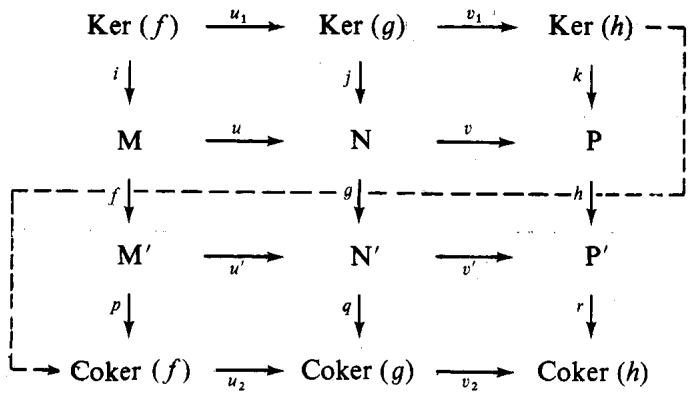
\includegraphics[keepaspectratio]{images/part001_0570902c.jpg}}

让我们证明 (i)。因为 \(u_{1}\) 与 \(v_{1}\) 分别同 \(u\) 和 \(v\) 到 \(\operatorname{Ker}(f)\) 与 \(\operatorname{Ker}(g)\) 上的限制具有相同的图像，我们有 \(v_{1} \circ u_{1} = 0\) 。我们有

\[
\operatorname{Ker} \left(v _ {1}\right) = \operatorname{Ker} (g) \cap \operatorname{Ker} (v) = \operatorname{Ker} (g) \cap \operatorname{Im} (u) = \operatorname{Im} (j) \cap \operatorname{Im} (u).
\]

但由命题1(i)，我们有 \(\operatorname{Ker}(v_1) = \operatorname{Im}(j \circ u_1) = \operatorname{Im}(u_1)\) 如果 \(u'\) 是单射。我们来证明 (ii)。由于 \(u_2\) 与 \(v_2\) 是由 \(u\) 和 \(v\) 通过取商得出的，显然 \(v_2 \circ u_2 = 0\) 。假设 \(v\) 是满射；由于 \(q\) 与 \(p\) 是满射，根据假设及命题 1 (ii)，我们有

\[
\begin{array}{r l} \operatorname{Ker} (v _ {2}) & = q (\operatorname{Ker} (v _ {2} \circ q)) = q (\operatorname{Ker} (v ^ {\prime}) + \operatorname{Im} (g)) = q (\operatorname{Ker} (v ^ {\prime})) \\ & = q (\operatorname{Im} (u ^ {\prime})) = \operatorname{Im} (q \circ u ^ {\prime}) = \operatorname{Im} (u _ {2} \circ p) = \operatorname{Im} (u _ {2}). \end{array}
\]

最后，我们来证明（iii）。对于 \(z \in \operatorname{Ker}(h)\) 存在 \(y \in \mathbf{N}\) 使得 \(v(y) = k(z)\) 因为 \(v\) 是满射；此外，我们有 \(v'(g(y)) = h(k(z)) = 0\) 因此存在唯一的 \(x' \in \mathbf{M}'\) 使得 \(u'(x') = g(y)\) 因为 \(u'\) 是单射。让我们证明元素 \(p(x') \in \operatorname{Coker}(f)\) 不依赖于元素 \(y \in \mathbf{N}\) ，只要它满足 \(v(y) = k(z)\) 。事实上，如果 \(y_1 \in \mathbf{N}\) 是另一个满足 \(v(y_1) = k(z)\) 的元素，我们有 \(y_1 = y + u(x)\) ，其中 \(x \in \mathbf{M}\) 。让我们证明，如果 \(x_1' \in \mathbf{M}'\) 满足 \(u'(x_1') = g(y_1)\) ，则 \(x_1' = x' + f(x)\) ；事实上，我们有 \(u'(x' + f(x)) = u'(x') + u'(f(x)) = g(y) + g(u(x)) = g(y + u(x)) = g(y_1)\) 最后，我们得出结论 \(p(x_1') = p(x') + p(f(x)) = p(x')\) 。因此我们可令 \(d(z) = p(x')\) ，并由此定义了一个映射 \(d: \operatorname{Ker}(h) \to \operatorname{Coker}(f)\) 。

如果现在 \(z_{1}, z_{2}\) 是 \(\operatorname{Ker}(h)\) 的元素，如果 \(\lambda_{1}, \lambda_{2} \in \mathbf{A}\) 和 \(z = \lambda_{1} z_{1} + \lambda_{2} z_{2}\) ，我们取元素 \(y_{1}\) 和 \(y_{2}\) 属于 \(\mathbf{N}\) ，使得 \(v(y_{1}) = k(z_{1})\) 和 \(v(y_{2}) = k(z_{2})\) ，并为 \(y \in \mathbf{N}\) 选取元素 \(\lambda_{1} y_{1} + \lambda_{2} y_{2}\) ；那么立即可以得出

\[
d (z) = \lambda_ {1} d (z _ {1}) + \lambda_ {2} d (z _ {2}),
\]

所以 d 是一个同态。

假设 \(z = v_1(t)\) 对于某个 \(t \in \operatorname{Ker}(g)\) ；我们将取 \(y \in \mathbf{N}\) 为元素 \(j(t)\) 。由于 \(g(j(t)) = 0\) ，我们得出结论 \(d(z) = 0\) ，因此 \(d \circ v_1 = 0\) 。反之，假设 \(d(z) = 0\) 。利用前面的记号，我们因此有 \(x' = f(x)\) ，其中 \(x \in M\) 。在这种情况下，我们有 \(g(y) = u'(f(x)) = g(u(x))\) ，或等价地 \(g(y - u(x)) = 0\) 。元素 \(y - u(x)\) 因此具有形式 \(j(n)\) 当 \(n \in \operatorname{Ker}(g)\) ，并且我们有

\[
k (z) = v (y) = v (u (x) + j (n)) = v (j (n)) = k \left(v _ {1} (n)\right);
\]

因为 \(k\) 是单射， \(z = v_{1}(n)\) ，这证明了序列(*)在 \(\operatorname{Ker}(h)\) 处是正合的。最后，我们仍有（使用相同的记号）

\[
u _ {2} (d (z)) = u _ {2} \left(p \left(x ^ {\prime}\right)\right) = q \left(u ^ {\prime} \left(x ^ {\prime}\right)\right) = q (g (y)) = 0 \quad \text {   hence   } \quad u _ {2} \circ d = 0.
\]

反之，假设一个元素 \(w = p(x')\) —— Coker \((f)\) 的元素 —— 满足

\[
u _ {2} (w) = u _ {2} \left(p \left(x ^ {\prime}\right)\right) = 0 \quad \left(\operatorname{with} x ^ {\prime} \in \mathbf {M} ^ {\prime}\right).
\]

我们因此有 \(q(u'(x')) = 0\) ，从而 \(u'(x') = g(y)\) 对于某个 \(y \in \mathbb{N}\) ；由于 \(v'(u'(x')) = 0\) ，我们有 \(v'(g(y)) = 0\) ，因此 \(h(v(y)) = 0\) ，换言之 \(v(y) = k(z)\) 对于某个 \(z \in \operatorname{Ker}(h)\) ，并且根据定义 \(w = d(z)\) ，这表明序列(*)在Coker( \(f\) )处是正合的。我们在(i)中看到它在Ker( \(g\) )处是正合的，在(ii)中看到它在Coker( \(g\) )处是正合的，这完成了(iii)的证明。

推论1. --- 假设图(4)是交换的且具有正合的行。则：

\begin{enumerate}
\def\labelenumi{(\roman{enumi})}
\item
  若 \(u'\) , \(f\) 和 \(h\) 是单射，则 \(g\) 是单射。
\item
  如果v、f和h是满射，则g是满射。
\end{enumerate}

断言 (i) 由命题 2 的断言 (i) 得出：事实上，我们有 \(\operatorname{Ker}(f) = 0\) 和 \(\operatorname{Ker}(h) = 0\) ，因此 \(\operatorname{Ker}(g) = 0\) 。

断言(ii)由命题2的断言(ii)得出：事实上，我们有Coker \(f\) = 0 且 Coker \(h\) = 0，因此 Coker \(g\) = 0.

推论 2. --- 假设图 (4) 是交换的且具有正合行。在这些条件下：

\begin{enumerate}
\def\labelenumi{(\roman{enumi})}
\item
  若g是单射，且f和v是满射，则h是单射。
\item
  若g是满射，且h与u'是单射，则f是满射。
\end{enumerate}

为了证明(i)，考虑该图表。

\[
\begin{array}{c c c c c} u (\mathbf {M}) & \xrightarrow {w} & \mathbf {N} & \xrightarrow {v} & \mathbf {P} \\ f ^ {\prime} \Big \downarrow & & g \Big \downarrow & & h \Big \downarrow \\ u ^ {\prime} (\mathbf {M} ^ {\prime}) & \xrightarrow {w ^ {\prime}} & \mathbf {N} ^ {\prime} & \xrightarrow {v ^ {\prime}} & \mathbf {P} ^ {\prime} \end{array}
\]

其中 \(f'\) 是与 \(g\) 到 \(u(\mathbf{M})\) 上的限制具有相同图像的映射， \(w\) 和 \(w'\) 为典范单射；显然该图表是交换的且行是正合的。此外 \(w'\) 是单射的，且根据假设 \(v\) 是满射；因此由命题2(iii)，我们有一个正合序列

\[
\operatorname{Ker} (g) \longrightarrow \operatorname{Ker} (h) \xrightarrow {d} \operatorname{Coker} \left(f ^ {\prime}\right);
\]

由于g是单射且 \(f'\) 是满射，因此我们有 Ker(h) = 0。

为证明(ii)，考虑如下图表。

\[
\begin{array}{c c c c c} \mathbf {M} & \stackrel {{u}} {{\longrightarrow}} & \mathbf {N} & \stackrel {{w}} {{\longrightarrow}} & v (\mathbf {N}) \\ f \Big \downarrow & & g \Big \downarrow & & h ^ {\prime} \Big \downarrow \\ \mathbf {M} ^ {\prime} & \stackrel {{u ^ {\prime}}} {{\longrightarrow}} & \mathbf {N} ^ {\prime} & \stackrel {{w ^ {\prime}}} {{\longrightarrow}} & v ^ {\prime} (\mathbf {N} ^ {\prime}) \end{array}
\]

此时 \(h'\) 是与 \(h\) 到 \(v(\mathbf{N})\) 上的限制具有相同图像的映射，且 \(w\) 和 \(w'\) 分别具有与 \(v\) 和 \(v'\) 相同的图像；此图表可交换且其行是正合的。此外 \(w\) 是满射，且根据假设 \(u'\) 是单射；因此由命题2(iii)，我们得到正合序列

\[
\operatorname{Ker} \left(h ^ {\prime}\right) \xrightarrow {d} \operatorname{Coker} (f) \longrightarrow \operatorname{Coker} (g);
\]

因为 \(g\) 是满射且 \(h'\) 是单射，因此我们有 Coker \((f) = 0\) 。

推论3（五引理）。——考虑一个A-模的交换图表

\[
\begin{array}{c c c c c c c c c} \mathbf {M} _ {1} & \xrightarrow {u _ {1}} & \mathbf {M} _ {2} & \xrightarrow {u _ {2}} & \mathbf {M} _ {3} & \xrightarrow {u _ {3}} & \mathbf {M} _ {4} & \xrightarrow {u _ {4}} & \mathbf {M} _ {5} \\ f _ {1} \Big \downarrow & & f _ {2} \Big \downarrow & & f _ {3} \Big \downarrow & & f _ {4} \Big \downarrow & & f _ {5} \Big \downarrow \\ \mathbf {M} _ {1} ^ {\prime} & \xrightarrow {u _ {1} ^ {\prime}} & \mathbf {M} _ {2} ^ {\prime} & \xrightarrow {u _ {2} ^ {\prime}} & \mathbf {M} _ {3} ^ {\prime} & \xrightarrow {u _ {3} ^ {\prime}} & \mathbf {M} _ {4} ^ {\prime} & \xrightarrow {u _ {4} ^ {\prime}} & \mathbf {M} _ {5} ^ {\prime} \end{array}
\]

其中的行是正合的。

\begin{enumerate}
\def\labelenumi{(\roman{enumi})}
\item
  若 \(f_{2}\) 和 \(f_{4}\) 是单射且 \(f_{1}\) 是满射，则 \(f_{3}\) 是单射。
\item
  若 \(f_{2}\) 和 \(f_{4}\) 都是满射且 \(f_{5}\) 是单射，则 \(f_{3}\) 是满射。
\end{enumerate}

特别地，如果 \(f_1, f_2, f_4\) 和 \(f_5\) 是同构，那么 \(f_3\) 也是。为证明 (i)，设 \(\tilde{\mathbf{M}}_2 = \text{Coker } (u_1), \tilde{\mathbf{M}}_2' = \text{Coker } (u_1')\) 并记 \(\tilde{f}_2: \tilde{\mathbf{M}}_2 \to \tilde{\mathbf{M}}_2'\) 由 \(f_2\) 推出的映射。由推论2(i)可知 \(\tilde{f}_2\) 是单射的。将推论1(i)应用于该图表

\[
\begin{array}{c c c c c} \tilde {\mathbf {M}} _ {2} & \xrightarrow {\tilde {u} _ {2}} & \mathbf {M} _ {3} & \xrightarrow {u _ {3}} & \mathbf {M} _ {4} \\ \tilde {f} _ {2} \Big \downarrow & & f _ {3} \Big \downarrow & & f _ {4} \Big \downarrow \\ \tilde {\mathbf {M}} _ {2} ^ {\prime} & \xrightarrow {\tilde {u} _ {2} ^ {\prime}} & \mathbf {M} _ {3} ^ {\prime} & \xrightarrow {u _ {3} ^ {\prime}} & \mathbf {M} _ {4} ^ {\prime} \end{array}
\]

其中 \(\tilde{u}_2\) 和 \(\tilde{u}_2'\) 是由 \(u_2\) 和 \(u_2'\) 得出的，我们看到 \(f_3\) 是单射。

为了证明(ii)，设 \(\tilde{\mathbf{M}}_{4} = \operatorname{Ker}(u_{4}), \tilde{\mathbf{M}}_{4}' = \operatorname{Ker}(u_{4}')\) 并记 \(\tilde{f}_{4}: \tilde{\mathbf{M}}_{4} \to \tilde{\mathbf{M}}_{4}'\) 由 \(f_{4}\) 诱导的映射。由推论2(ii)可知， \(\tilde{f}_{4}\) 是满射的。将推论1(ii)应用于该图表

\[
\begin{array}{c c c c c} \mathbf {M} _ {2} & \xrightarrow {u _ {2}} & \mathbf {M} _ {3} & \xrightarrow {\tilde {u} _ {3}} & \tilde {\mathbf {M}} _ {4} \\ f _ {2} \Big \downarrow & & f _ {3} \Big \downarrow & & \tilde {f} _ {4} \Big \downarrow \\ \mathbf {M} _ {2} ^ {\prime} & \xrightarrow {u _ {2} ^ {\prime}} & \mathbf {M} _ {3} ^ {\prime} & \xrightarrow {\tilde {u} _ {3} ^ {\prime}} & \tilde {\mathbf {M}} _ {4} ^ {\prime} \end{array}
\]

其中 \(\tilde{u}_3\) 和 \(\tilde{u}_3'\) 分别与 \(u_3\) 和 \(u_3'\) 具有相同的图像，我们看到 \(f_3\) 是满射。

\subsection{平坦模}

定义 1. —— 称 A-模 E 为平坦的，如果对于右 A-模与同态的每个正合序列，

\[
\mathbf {M} ^ {\prime} \xrightarrow {u} \mathbf {M} \xrightarrow {v} \mathbf {M} ^ {\prime \prime},\tag{11}
\]

由Z-线性映射构成的序列

\[
\mathbf {M} ^ {\prime} \otimes_ {\mathbf {A}} \mathrm{E} \xrightarrow {u \otimes 1} \mathbf {M} \otimes_ {\mathbf {A}} \mathrm{E} \xrightarrow {v \otimes 1} \mathbf {M} ^ {\prime \prime} \otimes_ {\mathbf {A}} \mathrm{E}\tag{12}
\]

是正合的。

命题 3. —— A-模 E 为平坦的，当且仅当对于每个右 A-模的单射 A-同态 \(u: \mathbf{M}' \to \mathbf{M}\) ，映射 \(u \otimes 1: \mathbf{M}' \otimes_{\mathbf{A}} \mathbf{E} \to \mathbf{M} \otimes_{\mathbf{A}} \mathbf{E}\) 是单射。

如果 E 是平坦的且 \(u: \mathbf{M}' \to \mathbf{M}\) 是单射，序列 \(0 \longrightarrow \mathbf{M}' \stackrel{u}{\longrightarrow} \mathbf{M}\) 是正合的，因此也有

序列 0 \(\longrightarrow\) M' \(\otimes_{\mathbf{A}}\) E \(\xrightarrow{u\otimes1}\) M \(\otimes_{\mathbf{A}}\) E，且 \(u\otimes1\) 是单射。反之，考虑正合序列（11）；设 M'\,' \(_{1}\) = v(M)，并令 i : M'\,' \(_{1}\) → M'\,' 为典范单射

和 \(p:\mathbf{M}\to\mathbf{M}_{1}^{\prime\prime}\) 为映射 \(m\mapsto v(m)\) 。序列 \(\mathbf{M}^{\prime}\xrightarrow{u}\mathbf{M}\xrightarrow{p}\mathbf{M}_{1}^{\prime\prime}\longrightarrow0\)

是正合的；由 II，第～58 页，命题 5，序列 \(\mathbf{M}' \otimes_{\mathbf{A}} \mathbf{E} \xrightarrow{u \otimes 1} \mathbf{M} \otimes_{\mathbf{A}} \mathbf{E} \xrightarrow{p \otimes 1} \mathbf{M}_{1}'' \otimes_{\mathbf{A}} \mathbf{E}\) 因此是正合的。此外，我们有 \(v = i \circ p\) ，因此 \((v \otimes 1) = (i \otimes 1) \circ (p \otimes 1)\) ；若 E 满足命题中的条件，则 \(i \otimes 1\) 是单射，因此

\[
\operatorname{Ker} (v \otimes 1) = \operatorname{Ker} (p \otimes 1) = \operatorname{Im} (u \otimes 1)
\]

且序列 (12) 是正合的。

命题4. ---（i）设 \((\mathbf{E}_i)_{i\in \mathbf{I}}\) 是 A-模的一个族， \(\mathrm{E} = \bigoplus_{i\in \mathbf{I}}\mathrm{E}_i\) 它们的直和

为使 A-模 E 是平坦的，其充要条件是每一个 \(E_{i}\) 都是平坦的。

\begin{enumerate}
\def\labelenumi{(\roman{enumi})}
\setcounter{enumi}{1}
\tightlist
\item
  设 I 是一个右有向预序集， \((\mathrm{E}_{\alpha}, f_{\beta\alpha})\) 是关于 I 的 A-模归纳系， \(E = \varinjlim E_{\alpha}\) 为其归纳极限。若每个 A-模 \(E_{\alpha}\) 是平坦的，则 E 是平坦的。
\end{enumerate}

设 \(M^{\prime} \rightarrow M \rightarrow M^{\prime\prime}\) 是右A-模的一个正合序列。

\begin{enumerate}
\def\labelenumi{(\roman{enumi})}
\item
  为使序列 \(\bigoplus_{i\in I}(\mathbf{M}^{\prime}\otimes_{\mathbf{A}}\mathbf{E}_{i})\to \bigoplus_{i\in I}(\mathbf{M}\otimes_{\mathbf{A}}\mathbf{E}_{i})\to \bigoplus_{i\in I}(\mathbf{M}^{\prime \prime}\otimes_{\mathbf{A}}\mathbf{E}_{i})\) 正合，必要且充分的是每个序列 \(\mathbf{M}^{\prime}\otimes_{\mathbf{A}}\mathbf{E}_{i}\to \mathbf{M}\otimes_{\mathbf{A}}\mathbf{E}_{i}\to \mathbf{M}^{\prime \prime}\otimes_{\mathbf{A}}\mathbf{E}_{i}\) 都正合（II，第 13 页，命题 7），这就证明了 (i)，因为 \(\oplus (\mathbf{M}\otimes_{\mathbf{A}}\mathbf{E}_{i})\) 典范地等同于 \(\mathbf{M}\otimes_{\mathbf{A}}\mathbf{E}\) （II，第 61 页，命题 7）。
\item
  根据假设，每个序列 \(\mathbf{M}' \otimes_{\mathbf{A}} \mathbf{E}_i \to \mathbf{M} \otimes_{\mathbf{A}} \mathbf{E}_i \to \dot{\mathbf{M}}'' \otimes_{\mathbf{A}} \mathbf{E}_i\) 都是正合的，因此序列 \(\mathbf{M}' \otimes_{\mathbf{A}} \mathbf{E} \to \mathbf{M} \otimes_{\mathbf{A}} \mathbf{E} \to \mathbf{M}'' \otimes_{\mathbf{A}} \mathbf{E}\) 也是正合的，因为取归纳极限与张量积可交换（II，第 93 页，命题 7）并保持正合性（II，第 91 页，命题 3）。
\end{enumerate}

例。--- 1) 显然 \(A_{s}\) 是一个平坦A-模；于是由命题4(i)可知，每个自由A-模，更一般地每个投射A-模，都是平坦的（另见II，第63页，推论6）。

* 反之，每个有限表示的平坦 A-模都是投射的（第 5 节）。 *

\begin{enumerate}
\def\labelenumi{\arabic{enumi})}
\setcounter{enumi}{1}
\item
  由命题 4 (ii)，每个作为自由 A-模的有向归纳系的归纳极限的 A-模都是平坦的。我们将在第 6 节证明一个逆命题。
\item
  若A是半单的，则每个A-模都是投射的（VIII，§5，第1节，命题1），从而是平坦的。
\item
  * 若A是阿廷局部环（不一定交换），则一个A-模是平坦的当且仅当它是自由的（AC II，§3，第2节，命题5的推论2）。 *
\item
  若A是整环，则A的分式域K是平坦A-模（II，第118页，命题27）。
\item
  * 在AC II和III中，我们将研究当A为交换环时平坦A-模的两个重要例子：分式环 \(S^{-1}\) A，以及当A为诺特环时，A关于J-adic拓扑的分离完备化。 *
\item
  设 \(a \in \mathbf{A}\) 使得映射 \(a_{\mathbf{A}}: x \mapsto ax\) 从 \(\mathbf{A}\) 到 \(\mathbf{A}\) 是单射（“ \(a\) 不是左零因子”）。如果 \(\mathbf{E}\) 是平坦 \(\mathbf{A}\) -模，则位似 \(a_{\mathbf{E}}\) 是单射，因为它等同于 \(a_{\mathbf{A}} \otimes 1: \mathbf{A}_{d} \otimes_{\mathbf{A}} \mathbf{E} \to \mathbf{A}_{d} \otimes_{\mathbf{A}} \mathbf{E}\) 。特别地，如果 \(\mathbf{A}\) 是整环，则每个平坦 \(\mathbf{A}\) -模都是无挠的。反之，如果 \(\mathbf{A}\) 是主理想环，则每个无挠 \(\mathbf{A}\) -模都是平坦的：事实上，如果 \(\mathbf{A}\) -模 \(\mathbf{E}\) 是无挠的，则 \(\mathbf{E}\) 的每个有限生成子模都是自由的（第七章，第4节，第4号，定理4的推论2），并且 \(\mathbf{E}\) 是平坦子模的有向递增并，因此是平坦的（命题4（ii））。
\item
  设 B 为一个环，且 \(\rho: \mathbf{A} \to \mathbf{B}\) 一个同态。若 E 是平坦的 A-模，则 B-模 \(\mathbf{E}_{(\mathbf{B})} = \mathbf{B} \otimes_{\mathbf{A}} \mathbf{E}\) 是平坦的。事实上，设 \(u: \mathbf{N}' \to \mathbf{N}\) 是右 B-模的一个单同态；则 \(u \otimes_{\mathbf{B}} 1_{\mathbf{E}_{(\mathbf{B})}}\) 典范地等同于同态 \(u \otimes_{\mathbf{A}} 1_{\mathbf{E}}: \mathbf{N}' \otimes_{\mathbf{A}} \mathbf{E} \to \mathbf{N} \otimes_{\mathbf{A}} \mathbf{E}\) ，若 E 是平坦的，则该同态是单的。
\item
  假设 \(\mathbf{A} = \mathbf{K}[\mathbf{X}, \mathbf{Y}]\) ，其中 \(\mathbf{K}\) 是一个域。则极大理想 \(m\) 由 \(\mathbf{X}\) 和 \(\mathbf{Y}\) 生成，它是一个无挠 A-模，但不是平坦的。事实上，考虑环 \(\mathbf{B} = \mathbf{A}/(\mathbf{Y})\) ，它同构于 \(\mathbf{K}[\mathbf{X}]\) ，因此是一个整环。B-模 \(m_{(B)}\) 同构于 \(m/Ym = (X, Y)/(XY, Y^2)\) ，其中 \(Y\) 的类是挠元。因此， \(m_{(B)}\) 不是平坦的B-模，从而 \(m\) 不是平坦的。
\item
  假设 A 是交换的。设 B 为代数 \(\mathbf{A}[\mathbf{X}_1, \ldots, \mathbf{X}_n] / (\mathbf{P})\) ，其中 P 是非零多项式。对于 A 的每个素理想 p，记 \(\kappa(p)\) 为整环 \(\mathbf{A} / p\) 的分式域， \(\mathbf{E}(p)\) 为代数 \(\kappa(p) [\mathbf{X}_1, \ldots, \mathbf{X}_n]\) ，并记 \(\mathbf{P}(p)\) 为 P 在典范映射下在 \(\mathbf{E}(p)\) 中的像。
\end{enumerate}

可以证明，要使 B 成为平坦的 A-模，只需 \(P(p) \neq 0\) 对 A 的每个素理想 p 成立。若 A 是整环，则此条件也是必要的。

* 用几何语言来说，考虑投影 \(\pi: \text{Spec}(B) \to \text{Spec}(A)\) 。对每个 \(p \in \text{Spec}(A)\) ，纤维 \(\pi^{-1}(p)\) 等同于子簇 \(V_p\) ，即仿射空间 \(\mathbf{A}_{\kappa(p)}^n = \text{Spec}(E(p))\) 中由 \(P(p)\) 所定义的子簇，而集合 \(F\) ——由使得该子簇为整个空间的 \(p\) （即使 \(P(p) = 0\) ）组成——是

Spec(A) 的闭子集。前述条件意味着该闭集为空，换言之，对每个 p，子簇 \(V_{p}\) 是 \(\mathbf{A}_{\kappa(p)}^{n}\) 中的一个超曲面。 *

\begin{enumerate}
\def\labelenumi{\arabic{enumi})}
\setcounter{enumi}{10}
\tightlist
\item
  设 S 和 X 为两个复解析空间，且 \(f: \mathbf{X} \to \mathbf{S}\) 为一个态射。我们说 \(f\) 在点 \(x\) （属于 \(\mathbf{X}\) ）处是平坦的，如果 \(\mathcal{O}_{\mathbf{X},x}\) 被视为 \(\mathcal{O}_{\mathbf{S},f(x)}\) -模（经由同态 \(f^{*}: \mathcal{O}_{\mathbf{S},f(x)} \to \mathcal{O}_{\mathbf{X},x}\) ）时是平坦的。\(\mathbf{X}\) 中使 \(f\) 平坦的点所成的集合是 \(\mathbf{X}\) 的一个开子集，并且 \(f\) 在这个开子集上的限制是一个开映射。如果 \(\mathbf{X}\) 和 \(\mathbf{S}\) 是连通的有限维解析流形，那么 \(f\) 是平坦的（在 \(\mathbf{X}\) 的每一点处）当且仅当 \(f(\mathbf{X})\) 在 \(\mathbf{S}\) 中是开的，并且纤维 \(f^{-1}(s)\) （对于 \(s \in f(\mathbf{X})\) ）都具有相同的维数。*
\end{enumerate}

\subsection{有限表示模}

A-模 E 的一个表示（或长度为 1 的表示）是一个正合序列

\[
\mathrm{L} _ {1} \rightarrow \mathrm{L} _ {0} \rightarrow \mathrm{E} \rightarrow 0\tag{13}
\]

其中 \(\mathbf{L}_0\) 和 \(\mathbf{L}_1\) 是自由 A-模。

每个 A-模 E 都有一个表示。事实上，我们知道（II，第 27 页，命题 20）存在一个满同态 \(u: \mathbf{L}_0 \to \mathbf{E}\) ，其中 \(\mathbf{L}_0\) 是自由的；如果 R 是 \(u\) 的核，同样存在一个满同态 \(v: \mathbf{L}_1 \to \mathbf{R}\) ，其中 \(\mathbf{L}_1\) 是自由的。如果将 \(v\) 视为从 \(\mathbf{L}_1\) 到 \(\mathbf{L}_0\) 的同态，序列 \(\mathbf{L}_1 \xrightarrow{v} \mathbf{L}_0 \xrightarrow{u} \mathbf{E} \longrightarrow 0\) 依定义是正合的，因此我们的断言成立。

若 \(\rho: A \to B\) 是一个环同态，那么 \(E\) 的每个表示 (13) 给出 \(E_{(B)} = B \otimes_A E\) 的一个表示：

\[
\mathbf {B} \otimes_ {\mathbf {A}} \mathrm{L} _ {1} \rightarrow \mathbf {B} \otimes_ {\mathbf {A}} \mathrm{L} _ {0} \rightarrow \mathbf {B} \otimes_ {\mathbf {A}} \mathrm{E} \rightarrow 0\tag{14}
\]

这由 II，第 58 页，命题 5 以及 \(\mathbf{B} \otimes_{\mathbf{A}} \mathbf{L}\) 当 L 是自由模时是自由 B-模这一事实得出。

称模 E 的一个表示 (13) 是有限的，如果自由模 \(L_{0}\) 和 \(L_{1}\) 有有限基。显然，如果表示 (13) 是有限的，那么表示 (14) 也是有限的。称 E 为有限表示的 A-模，如果它有一个有限表示。

命题5. --- (i) 每个具有有限表示的模都是有限生成的。

\begin{enumerate}
\def\labelenumi{(\roman{enumi})}
\setcounter{enumi}{1}
\item
  若A是左诺特环，则每个有限生成的A-模都有有限表示。
\item
  每个有限生成的投射模都具有有限表示。
\end{enumerate}

断言（i）由定义直接得出。假设A是左诺特的，且E是有限生成的。那么存在一个满同态 \(u: L_0 \to E\) ，其中 \(L_0\) 是具有有限基的自由 A-模；\(u\) 的核 R 是有限生成的，因此存在一个满同态 \(v: L_1 \to R\) ，其中 \(L_1\) 是具有有限基的自由模，并且正合序列 \(L_1 \xrightarrow{v} L_0 \xrightarrow{u} E \longrightarrow 0\) 是E的一个有限表示；由此得(ii)。

最后，假设 E 是一个有限生成的投射模；那么它是有限生成自由模 \(L_{0}\) 的一个直和项（II，第 40 页，推论 1）；满同态 \(L_{0} \rightarrow E\) 的核 R 则同构于 \(L_{0}\) 的一个商，因此是有限生成的，并像上面那样完成证明。

命题6. --- 设A是一个环，E是一个有限表示的A-模。对于每个正合序列

\[
0 \longrightarrow \mathrm{F} \stackrel {j} {\longrightarrow} \mathrm{G} \stackrel {p} {\longrightarrow} \mathrm{E} \longrightarrow 0
\]

其中G是有限生成的，模F也是有限生成的。

设 \(L_{1} \xrightarrow{r} L_{0} \xrightarrow{s} E \longrightarrow 0\) 是一个有限表示；如果 \((e_{i})\) 是 \(L_{0}\) 的一组基，则对每个 i 存在一个元素 \(g_{i} \in G\) 使得 \(p(g_{i}) = s(e_{i})\) ；同态 \(u : L_{0} \to G\) （对一切 i 满足 \(u(e_{i}) = g_{i}\) ）因而满足 \(s = p \circ u\) 。由于 \(s \circ r = 0\) ，我们有 \(u(r(L_{1})) \subset \operatorname{Ker} p\) ，并且由于 Ker p 同构于 F，我们看到存在一个同态 \(v : L_{1} \to F\) 使得图表

\[
\begin{array}{c c c c c c c} L _ {1} & \xrightarrow {r} & L _ {0} & \xrightarrow {s} & E & \longrightarrow & 0 \\ v \Big \downarrow & & u \Big \downarrow & & ^ {1 _ {E}} \Big \downarrow \\ F & \xrightarrow {} _ {j} & G & \xrightarrow {} _ {p} & E & \longrightarrow & 0 \end{array}
\]

是交换的。由于 j 是单射且 s 是满射，可以应用 X 第 4 页的命题 2，换言之存在一个正合序列

\[
\operatorname{Ker} 1 _ {\mathrm{E}} \xrightarrow {d} \text { Coker } v \longrightarrow \text { Coker } u \longrightarrow \text { Coker } 1 _ {\mathrm{E}}.
\]

这表明 Coker v 同构于 \(\mathrm{G}/u(\mathrm{L}_{0})\) ，而根据假设它是有限生成的。此外，我们还有正合序列

\[
0 \rightarrow v (\mathbf {L} _ {1}) \rightarrow \mathrm{F} \rightarrow \text { Coker } v \rightarrow 0
\]

并且由于 \(v(\mathbf{L}_1)\) 和Coker \(v\) 是有限生成的，所以 F（II，第 17 页，推论 5）也是有限生成的。

命题 7. —— 设 M 是一个 A-模。存在一个右有向有序集 I 和一个相对于 I 的、由有限表示 A-模构成的归纳系（M \(_{\alpha}\) , φ \(_{\beta\alpha}\) ），使得 M 同构于 lim M \(_{\alpha}\) 。若 M 具有由 n 个元素组成的生成族，则可假定 M \(_{\alpha}\)

亦然。考虑一个表示

\[
\mathrm{A} _ {s} ^ {(\mathrm{K})} \xrightarrow {u} \mathrm{A} _ {s} ^ {(\mathrm{L})} \xrightarrow {v} \mathrm{M} \longrightarrow 0;
\]

设 I 为由对 \(\alpha = (\mathbf{K}', \mathbf{L}')\) 组成的集合，其中 \(\mathbf{K}'\) （相应地， \(\mathbf{L}'\) ）是 \(\mathbf{K}\) （相应地 L）的有限子集，使得 \(u\) 诱导出映射 \(u_{\alpha}\) ，它把子模 \(\mathbf{A}_s^{\mathbf{K}'}\) （\(\mathbf{A}_s^{(\mathbf{K})}\) 的子模）映入子模 \(\mathbf{A}_s^{\mathbf{L}'}\) （\(\mathbf{A}_s^{(\mathbf{L})}\) 的子模）；对于 \(\alpha \in \mathbf{I}\) ，设 \(\mathbf{M}_{\alpha}\) 为 \(u_{\alpha}\) 的余核，并设 \(v_{\alpha}: \mathbf{A}_s^{\mathbf{L}'} \to \mathbf{M}_{\alpha}\) 为典范映射，从而我们有一个行正合的交换图：

\[
\mathrm{A} _ {s} ^ {(\mathrm{K})} \xrightarrow {u} \mathrm{A} _ {s} ^ {(\mathrm{L})} \xrightarrow {i} \mathrm{M} \longrightarrow 0
\]

\[
i _ {\alpha} \uparrow , \quad j _ {\alpha} \uparrow , \quad f _ {\alpha} \uparrow
\]

\[
\mathrm{A} _ {s} ^ {\mathrm{K} ^ {\prime}} \xrightarrow {u _ {\alpha}} \mathrm{A} _ {s} ^ {\mathrm{L} ^ {\prime}} \xrightarrow {v _ {\alpha}} \mathrm{M} _ {\alpha} \longrightarrow 0,
\]

其中 \(i_{\alpha}\) 和 \(j_{\alpha}\) 是典范单射，而 \(f_{\alpha}\) 是由 \(j_{\alpha}\) 通过取商得出的。按以下关系给集合 I 排序：

\[
\alpha = \left(\mathrm{K} ^ {\prime}, \mathrm{L} ^ {\prime}\right) \leqslant \beta = \left(\mathrm{K} ^ {\prime \prime}, \mathrm{L} ^ {\prime \prime}\right) \quad \text { if } \quad \mathrm{K} ^ {\prime} \subset \mathrm{K} ^ {\prime \prime}, \quad \mathrm{L} ^ {\prime} \subset \mathrm{L} ^ {\prime \prime};
\]

当 \(\alpha \leqslant \beta\) ，设 \(\varphi_{\beta \alpha}: \mathbf{M}_{\alpha} \to \mathbf{M}_{\beta}\) 为由 \(\mathbf{A}_s^{L'}\) 到 \(\mathbf{A}_s^{L''}\) 的包含映射通过取商得出的同态。于是可直接验证有序集 I 是有向的，且 \((\mathbf{M}_{\alpha}, \varphi_{\beta \alpha})\) 是 A-模的归纳系， \((\varphi_{\alpha})\) 是 A-同态的归纳系。取归纳极限，得到一个交换图

\[
\begin{array}{c c c c c} \mathbf {A} _ {s} ^ {(\mathbf {K})} & \stackrel {{u}} {{\longrightarrow}} & \mathbf {A} _ {s} ^ {(L)} & \stackrel {{v}} {{\longrightarrow}} & \mathbf {M} \\ i \uparrow & & j \uparrow & & \varphi \uparrow \\ \underline {{\lim}} \mathbf {A} _ {s} ^ {\mathbf {K} ^ {\prime}} & \longrightarrow & \underline {{\lim}} \mathbf {A} _ {s} ^ {\mathbf {L} ^ {\prime}} & \longrightarrow & \underline {{\lim}} \mathbf {M} _ {\alpha} \longrightarrow 0; \end{array}\tag{15}
\]

此图的行是正合的（II，p.～91，命题 3）；由于 i 和 j 是双射，φ 也是双射（X，p.～7，推论 3），由此得命题。

\subsection{有限表现模的同态}

设 E 为 A-模。若 I 是有向的预序集，且 \((\mathbf{G}_{i}, u_{ji})\) 是相对于 I 的 A-模归纳系，则典范映射 \(G_{i} \to \varinjlim G_{i}\) 诱导同态 \(\operatorname{Hom}_{\mathbf{A}}(\mathbf{E}, \mathbf{G}_{i}) \to \operatorname{Hom}_{\mathbf{A}}(\mathbf{E}, \varinjlim \mathbf{G}_{i})\) 从而得到一个称为典范的同态

\[
\varinjlim_ {i \in \mathrm{I}} \operatorname{Hom} _ {\mathrm{A}} (\mathrm{E}, \mathrm{G} _ {i}) \rightarrow \operatorname{Hom} _ {\mathrm{A}} (\mathrm{E}, \varinjlim_ {i \in \mathrm{I}} \mathrm{G} _ {i}).\tag{16}
\]

设 B 为另一个环，F 为 B-模，G 为 (A, B)-双模；我们在 II，p.～75 中定义了一个典范同态：

\[
\operatorname{Hom} _ {\mathbf {A}} (\mathrm{E}, \mathrm{G}) \otimes_ {\mathbf {B}} \mathrm{F} \rightarrow \operatorname{Hom} _ {\mathbf {A}} (\mathrm{E}, \mathrm{G} \otimes_ {\mathbf {B}} \mathrm{F}).\tag{17}
\]

命题 8. --- a) 若 A-模 E 是有限生成的（相应地有限表现的），则典范同态 (16) 是单射（相应地双射）。

\begin{enumerate}
\def\labelenumi{\alph{enumi})}
\setcounter{enumi}{1}
\tightlist
\item
  假设 B-模 F 是平坦的；若 A-模 E 是有限生成的（相应地有限表示的），则典范同态 (17) 是单射（相应地双射）。我们以 b) 为例证明，a) 的证明类似。将 A、B、F、G 视为固定的，并对每个右 A-模 E，令
\end{enumerate}

\[
\mathrm{T} (\mathrm{E}) = \operatorname{Hom} _ {\mathrm{A}} (\mathrm{E}, \mathrm{G}) \otimes_ {\mathrm{B}} \mathrm{F}, \quad \mathrm{T} ^ {\prime} (\mathrm{E}) = \operatorname{Hom} _ {\mathrm{A}} (\mathrm{E}, \mathrm{G} \otimes_ {\mathrm{B}} \mathrm{F})
\]

并记 \(\nu_{\mathbf{E}}\) 为同态 (17)；对每个右 A-模同态 \(v: \mathbf{E} \to \mathbf{E}'\) ，令 \(\mathbf{T}(v) = \operatorname{Hom}(v, 1_{\mathbf{G}}) \otimes 1_{\mathbf{F}}\) 和 \(\mathbf{T}'(v) = \operatorname{Hom}(v, 1_{\mathbf{G}} \otimes 1_{\mathbf{F}})\) 。

设 \(L_{1} \xrightarrow{v} L_{0} \xrightarrow{w} E \to 0\) 为 E 的一个表示；我们假设自由模 \(L_{0}\) （相应地自由模 \(L_{0}\) 和 \(L_{1}\) ）是有限生成的。图

\[
\begin{array}{c} 0 \to \mathrm{T(E)} \xrightarrow {\mathrm{T(w)}} \mathrm {T(L_ {0})} \xrightarrow {\mathrm{T(v)}} \mathrm {T(L_ {1})} \\ v _ {\mathrm{E}} \Big \downarrow \qquad \qquad \qquad \qquad \qquad \qquad \qquad \qquad \qquad \qquad \qquad \qquad \qquad \qquad \qquad \qquad \qquad \qquad \qquad \qquad \qquad \qquad \qquad \qquad \qquad \qquad \qquad \qquad \qquad \qquad \qquad \qquad \qquad \qquad 0 \to \mathrm {T^ {\prime} (E)} \xrightarrow [ \mathrm {T^ {\prime} (w)} ]{} \mathrm {T^ {\prime} (L_ {0})} \xrightarrow [ \mathrm {T^ {\prime} (v)} ]{} \mathrm {T^ {\prime} (L_ {1})} \end{array}\tag{18}
\]

是交换的，且其第二行是正合的（II，p.～36，定理 1）；此外，序列

\[
0 \rightarrow \operatorname{Hom} _ {\mathbf {A}} (\mathrm{E}, \mathrm{G}) \rightarrow \operatorname{Hom} _ {\mathbf {A}} (\mathrm{L} _ {0}, \mathrm{G}) \rightarrow \operatorname{Hom} _ {\mathbf {A}} (\mathrm{L} _ {1}, \mathrm{G})
\]

是正合的（同上引），且由于 F 是平坦的，(18) 的第一行也是正合序列（X，p.～8，定义 1）。既然如此，我们知道 \(v_{L_0}\) 是双射（相应地 \(v_{L_0}\) 和 \(v_{L_1}\) 是双射）（II，第 75 页，命题 2）。若仅假设 \(v_{L_0}\) 是双射，则由 (18) 可知 \(v_{L_0} \circ T(w) = T'(w) \circ v_E\) 是单射，因此 \(v_E\) 也是单射。若假设 \(v_{L_0}\) 和 \(v_{L_1}\) 二者都是双射，则由 X，第 6 页的推论 2 (ii) 可推出 \(v_E\) 是满射，而由于我们刚刚看到 \(v_E\) 是单射，故它是双射。

推论. --- 每个有限表现的平坦模都是投射的。

事实上，设 E 为有限表示的平坦 A-模。将 (b) 应用于情形 \(\mathbf{B} = \mathbf{A}\) , \(\mathbf{G} = {}_{\mathrm{s}}\mathbf{A}_{\mathrm{d}}\) , \(\mathbf{F} = \mathbf{E}\) ，我们看到典范同态

\[
\operatorname{Hom} _ {\mathbf {A}} (\mathbf {E}, \mathbf {A}) \otimes_ {\mathbf {A}} \mathbf {E} \rightarrow \operatorname{Hom} _ {\mathbf {A}} (\mathbf {E}, \mathbf {E})
\]

是满射。这意味着 E 是投射的（II，p.～77，注记 1）。

由前述推论和 X，第 10 页的命题 5，有限表示的平坦模与有限生成的投射模是同一类模。另一方面，存在有限生成的平坦模不是有限表示的，因此不是投射的（参见 X，第 170 页，习题 17；但另见 X，第 169 页，习题 13 和 14）。

\subsection{平坦模的结构}

引理 2. --- 设 I 为右有向有序集， \((\mathrm{E}_{\alpha}, \varphi_{\beta\alpha})\) 是相对于 I 的集合归纳系，E 为其归纳极限， \(\varphi_{\alpha}: E_{\alpha} \to E\) , \(\alpha \in I\) 为典范映射。设 \(f: I \to I\) 为一个映射使得 \(f(\alpha) > \alpha\) 当 \(\alpha \in I\) ，并假设对每个 \(\alpha \in I\) ，给定一个集合 \(L_{\alpha}\) 及映射 \(u_{\alpha}: E_{\alpha} \to L_{\alpha}\) 和 \(v_{\alpha}: L_{\alpha} \to E_{f(\alpha)}\) ，使得 \(v_{\alpha} \circ u_{\alpha}' = \varphi_{f(\alpha),\alpha}\) 。设 J 为通过赋予 I 关系“ \(\alpha \leqslant \beta\) 如果 \(\alpha = \beta\) 或 \(f(\alpha) \leqslant \beta\) ”而得到的有序集。若 \(\alpha\) , \(\beta \in J\) 且 \(\alpha \leqslant \beta\) ，设 \(\psi_{\beta\alpha}: L_{\alpha} \to L_{\beta}\) 为满足 \(\psi_{\beta\alpha} = Id\) 如果 \(\alpha = \beta\) , \(\psi_{\beta\alpha} = u_{\beta} \circ \varphi_{\beta,f(\alpha)} \circ v_{\alpha}\) 如果 \(f(\alpha) \leqslant \beta\) 如果 \(\alpha \in J\) ，设 \(\psi_{\alpha}: L_{\alpha} \to E\) 为映射 \(\varphi_{f(\alpha)} \circ v_{\alpha}\) 。则有序集 J 是有向的， \((L_{\alpha}, \psi_{\beta\alpha})\) 是相对于 J 的归纳系， \((\psi_{\alpha})\) 是映射的归纳系，且映射 \(\psi: \varinjlim L_{\alpha} \to E\) （由诸 \(\psi_{\alpha}\) 得出）是双射。

显然 J 是有向的。若 \(\alpha\) , \(\beta \in J\) 且 \(\alpha < \beta\) ，我们有

\[
\begin{array}{r l} \psi_ {\beta} \circ \psi_ {\beta \alpha} & = \varphi_ {f (\beta)} \circ v _ {\beta} \circ u _ {\beta} \circ \varphi_ {\beta , f (\alpha)} \circ v _ {\alpha} \\ & = \varphi_ {f (\beta)} \circ \varphi_ {f (\beta), \beta} \circ \varphi_ {\beta , f (\alpha)} \circ v _ {\alpha} = \varphi_ {f (\alpha)} \circ v _ {\alpha} = \psi_ {\alpha}; \end{array}
\]

同样地，如果 \(\alpha\) , \(\beta\) , \(\gamma \in J\) 且 \(\alpha < \beta < \gamma\) ，我们有

\[
\begin{array}{r l} \psi_ {\gamma \beta} \circ \psi_ {\beta \alpha} & = u _ {\gamma} \circ \varphi_ {\gamma , f (\beta)} \circ v _ {\beta} \circ u _ {\beta} \circ \varphi_ {\beta , f (\alpha)} \circ v _ {\alpha} \\ & = u _ {\gamma} \circ \varphi_ {\gamma , f (\beta)} \circ \varphi_ {f (\beta), \beta} \circ \varphi_ {\beta , f (\alpha)} \circ v _ {\alpha} = u _ {\gamma} \circ \varphi_ {\gamma , f (\alpha)} \circ v _ {\alpha} = \psi_ {\gamma \alpha}. \end{array}
\]

让我们证明最后一个断言：对于每个 \(\alpha \in J\) ，我们有

\[
\psi_ {\alpha} \circ u _ {\alpha} = \varphi_ {f (\alpha)} \circ v _ {\alpha} \circ u _ {\alpha} = \varphi_ {f (\alpha)} \circ \varphi_ {f (\alpha), \alpha} = \varphi_ {\alpha},
\]

因此 \(\varphi_{\alpha}(\mathrm{E}_{\alpha}) = \psi_{\alpha}(u_{\alpha}(\mathrm{E}_{\alpha})) \subset \psi_{\alpha}(\mathrm{L}_{\alpha})\) ，且 \(\psi\) 是满射。设 \(\alpha \in \mathbf{J}\) 并设 \(x, y \in \mathrm{L}_{\alpha}\) 且 \(\psi_{\alpha}(x) = \psi_{\alpha}(y)\) ，即 \(\varphi_{f(\alpha)}(v_{\alpha}(x)) = \varphi_{f(\alpha)}(v_{\alpha}(y))\) ；存在 \(\beta \in \mathrm{I}\) , \(\beta \geqslant f(\alpha)\) 使得

\[
\varphi_ {\beta , f (\alpha)} (v _ {\alpha} (x)) = \varphi_ {\beta , f (\alpha)} (v _ {\alpha} (y)),
\]

因此

\[
\psi_ {\beta , \alpha} (x) = u _ {\beta} (\varphi_ {\beta , f (\alpha)} (v _ {\alpha} (x))) = u _ {\beta} (\varphi_ {\beta , f (\alpha)} (v _ {\alpha} (y))) = \psi_ {\beta , \alpha} (y).
\]

且ψ是单射。

定理1（D. Lazard）。——对于每个A-模E，以下条件等价：

\begin{enumerate}
\def\labelenumi{(\roman{enumi})}
\item
  E是平坦的。
\item
  对于每个有限表示的A-模P，典范同态
\end{enumerate}

\[
\operatorname{Hom} _ {\mathbf {A}} (\mathrm{P}, \mathrm{A}) \otimes_ {\mathbf {A}} \mathrm{E} \rightarrow \operatorname{Hom} _ {\mathbf {A}} (\mathrm{P}, \mathrm{E})
\]

是满射。

\begin{enumerate}
\def\labelenumi{(\roman{enumi})}
\setcounter{enumi}{2}
\item
  对于每个有限表示的 A-模 P 以及每个同态 \(u : P \to E\) ，存在一个有限生成的自由 A-模 L 以及同态 \(v : P \to L\) 和 \(w : L \to E\) ，使得 \(u = w \circ v\) 。
\item
  存在一个有向有序集 J，一个由有限生成自由模构成的归纳系 \((\mathbf{L}_{j})_{j\in\mathbf{J}}\) 以及一个从 E 到 lim \(L_{j}\) 的同构。
\item
  (iv) \(\Rightarrow\) (i)：这由X的命题4(ii)（第8页）得出。
\item
  (i) \(\Rightarrow\) (ii)：这由X的命题8b)得出，见第12页。
\item
  (ii) \(\Rightarrow\) (iii)：设 P 是有限表示的 A-模，且 \(u: \mathbf{P} \to \mathbf{E}\) 的一个同态；由 (ii)，存在 \(v_1, \ldots, v_n \in \mathrm{Hom}_{\mathbf{A}}(\mathbf{P}, \mathbf{A})\) , \(w_1, \ldots, w_n \in \mathbf{E}\) 使得 \(u(x) = \sum v_i(x) w_i\) 对所有 \(x \in \mathbf{P}\) 成立；若 \(v: \mathbf{P} \to \mathbf{A}^n\) 是分量为 \((v_i)\) 的同态，而 \(w: \mathbf{A}^n \to \mathbf{E}\) 是同态 \((a_i) \mapsto \sum a_i w_i\) ，则我们确实有 \(u = w \circ v\) 。
\item
  (iii) \(\Rightarrow\) (iv)：假设(iii)成立，并设 \((\mathbf{E}_{\alpha},\varphi_{\beta ,\alpha})\) 是一个归纳系，相对于有向集I，由有限表示的A-模组成，其归纳极限为E（X，第11页，命题7）。如有必要，将I替换为字典序积I × N，其中 \(E_{(\alpha,n)} = E_{\alpha}\) 对每个n成立，我们可以假设I没有最大元素。对每个 \(\alpha \in I\) ，设 \(L_{\alpha}\) 为一个有限生成的自由A-模，并且 \(u_{\alpha}: E_{\alpha} \to L_{\alpha}, v_{\alpha}': L_{\alpha} \to E\) 为同态，使得 \(v_{\alpha}' \circ u_{\alpha}\) 是典范映射 \(\varphi_{\alpha}\) （从 \(E_{\alpha}\) 到 E 中）；由于 \(L_{\alpha}\) 是有限生成且自由的，且 I 没有最大元，存在一个指标 \(\beta > \alpha\) 和一个同态 \(v_{\alpha}'': L_{\alpha} \to E_{\beta}\) 使得 \(v_{\alpha}' = \varphi_{\beta} \circ v_{\alpha}''\) ；由于 \(\varphi_{\beta} \circ v_{\alpha}'' \circ u_{\alpha} = \varphi_{\beta} \circ \varphi_{\beta,\alpha}\) 并且由于 \(E_{\alpha}\) 是有限表示的，根据X第12页命题8a），存在 \(\gamma \geqslant \beta\) 使得 \(\varphi_{\gamma\beta} \circ v_{\alpha}'' \circ u_{\alpha} = \varphi_{\gamma\beta} \circ \varphi_{\beta\alpha} = \varphi_{\gamma\alpha}\) ；令 \(\gamma = f(\alpha)\) ，并设 \(v_{\alpha}\) 为同态 \(\varphi_{\gamma\beta} \circ v_{\alpha}''\) （从 \(L_{\alpha}\) 到 \(E_{f(\alpha)}\) 中），我们有 \(v_{\alpha} \circ u_{\alpha} = \varphi_{f(\alpha),\alpha}\) ，于是我们可以应用引理2，从而得到(iv)。
\end{enumerate}

推论。—— 设A是交换的。对于每个平坦的A-模E，A-模 \(\mathbf{T}(\mathrm{E}),\mathbf{S}(\mathrm{E}),\symbf{\Lambda}(\mathrm{E}),\mathbf{T}^{n}(\mathrm{E}),\mathbf{S}^{n}(\mathrm{E}),\symbf{\Lambda}^{n}(\mathrm{E})\) 是平坦的。

事实上，E 是一个有向系 \((\mathbf{L}_{j})\) 的归纳极限，其中该系由有限生成的自由 A-模组成，因此 \(\mathbf{T}(\mathbf{E})\) (相应地， \(\mathbf{S}(\mathbf{E})\) ，等等）是自由 A-模的有向系的归纳极限 \(\mathbf{T}(\mathbf{L}_{j})\) (相应地， \(\mathbf{S}(\mathbf{L}_{j})\) ，等等），因此是平坦的（参见III，第61页，命题6，第62页，定理1，第73页，命题8，第75页，定理1，第83页，命题9，以及第86页，定理1）。

注记. --- 在 (ii) 中考虑一个有限表示 \(A_{s}^{J} \xrightarrow{c} A_{s}^{I} \to P \to 0\) ，我们便得到条件 (ii')，它仍与前面的条件等价：

(ii') 对由 A 中元素组成的每个有限矩阵 \((c_{ij})_{i\in I,j\in J}\) ，每个解

\[
\pmb {e} = (e _ {i}) _ {i \in \mathbf {I}} \in \mathrm{E} ^ {\mathbf {I}}
\]

（即线性齐次方程组

\[
\sum_ {i \in \mathbf {I}} c _ {i j} e _ {i} = 0, \quad j \in \mathrm{J},
\]

的解）都可以写成 \(b_{1}z_{1}+\cdots+b_{n}z_{n}\) ，其中 \(b_{1},\ldots,b_{n}\in E\) ，并且其中，对于 \(r=1,\ldots,n\) , \(z_{r}=(z_{r,i})_{i\in I}\) 是 \(A^{I}\) 中下述方程组的解

\[
\sum_ {i \in \mathbf {I}} z _ {r, i} c _ {i j} = 0, \quad j \in \mathrm{J}.
\]

\subsection{内射模}

定义2. --- 称A-模E为内射的，如果对每个由A-模及同态构成的正合序列

\[
\mathbf {M} ^ {\prime} \xrightarrow {u} \mathbf {M} \xrightarrow {v} \mathbf {M} ^ {\prime \prime},\tag{19}
\]

由Z-线性映射构成的序列

\[
\operatorname{Hom} _ {\mathbf {A}} \left(\mathbf {M} ^ {\prime \prime}, \mathbf {E}\right) \xrightarrow {\operatorname{Hom} _ {\mathbf {A}} (v , 1)} \operatorname{Hom} _ {\mathbf {A}} (\mathbf {M}, \mathbf {E}) \xrightarrow {\operatorname{Hom} _ {\mathbf {A}} (u , 1)} \operatorname{Hom} _ {\mathbf {A}} \left(\mathbf {M} ^ {\prime}, \mathbf {E}\right)\tag{20}
\]

是正合的。

引理3. --- 对于A-模E为内射的，当且仅当对每个单射的 A-线性映射 u : M' → M，映射

\[
\operatorname{Hom} _ {\mathbf {A}} (u, 1): \operatorname{Hom} _ {\mathbf {A}} (\mathrm{M}, \mathrm{E}) \rightarrow \operatorname{Hom} _ {\mathbf {A}} (\mathrm{M} ^ {\prime}, \mathrm{E})
\]

是满射。

若E是内射的且若 \(u: \mathbf{M}' \to \mathbf{M}\) 是单射的，则序列 \(0 \to \mathbf{M}' \xrightarrow{u} \mathbf{M}\) 是正合的，因此序列 Hom (M, E) \(\xrightarrow{\text{Hom}(u,1)}\) Hom ( \(\mathbf{M}'\) , E) \(\to 0\) 是正合的，且 Hom ( \(u,1\) ) 是满射。反之，考虑正合序列 (19)；设 \(\mathbf{M}_{1}'' = v(\mathbf{M})\) 并设 \(i: \mathbf{M}_{1}'' \to \mathbf{M}''\) 为典范单射， \(p: \mathbf{M} \to \mathbf{M}_{1}''\) 为映射 \(m \mapsto v(m)\) 。序列 \(\mathbf{M}' \xrightarrow{u} \mathbf{M} \xrightarrow{p} \mathbf{M}_{1}'' \to 0\) 是正合的；由 II，第～36 页，定理 1，序列

\[
\operatorname{Hom} _ {\mathbf {A}} \left(\mathrm{M} _ {1} ^ {\prime \prime}, \mathrm{E}\right) \xrightarrow {\operatorname{Hom} (p , 1)} \operatorname{Hom} _ {\mathbf {A}} (\mathrm{M}, \mathrm{E}) \xrightarrow {\operatorname{Hom} (u , 1)} \operatorname{Hom} _ {\mathbf {A}} \left(\mathrm{M} ^ {\prime}, \mathrm{E}\right)
\]

是正合的。此外，我们有 Hom \((v, 1) = \text{Hom } (p, 1) \circ \text{Hom } (i, 1)\) 。若 E 满足引理的条件，则 Hom \((i, 1)\) 是满射，因此 Hom \((v, 1)\) 的像也是 Hom \((p, 1)\) 的像，且序列 (20) 是正合的。

注记. --- 设 E 是一个内射 A-模， \(u: \mathbf{M}' \to \mathbf{M}\) 和 \(f: \mathbf{M}' \to \mathbf{E}\) 为 A-模的同态。若 \(\operatorname{Ker} u \subset \operatorname{Ker} f\) ，则存在一个同态 \(g: \mathbf{M} \to \mathbf{E}\) 使得 \(g \circ u = f\) 。这实际上由前述内容推出，将其应用于单射同态 \(\mathbf{M}' / \operatorname{Ker} u \to \mathbf{M}\) （由 \(u\) 得出）。

命题 9. --- 设 \((\mathbf{E}_i)_{i\in I}\) 是 A-模的一个族， \(\mathbf{E} = \prod \mathbf{E}_i\) 它们的积。对于 A-模 E 为内射的，必要且充分条件是每个 \(\mathbf{E}_i\) 都是内射的。

设 \(u: \mathbf{M}' \to \mathbf{M}\) 是 A-模的一个内射同态。对于积同态 \(\prod_{i \in I} \operatorname{Hom}_{\mathbf{A}}(\mathbf{M}, \mathbf{E}_i) \to \prod_{i \in I} \operatorname{Hom}_{\mathbf{A}}(\mathbf{M}', \mathbf{E}_i)\) 为满射的，必要且充分条件是每个同态 \(\operatorname{Hom}_{\mathbf{A}}(\mathbf{M}, \mathbf{E}_i) \to \operatorname{Hom}_{\mathbf{A}}(\mathbf{M}', \mathbf{E}_i)\) 都是满射的（II，第～10 页，命题 5）；这证明了该命题，因为 \(\prod_{i \in I} \operatorname{Hom}_{\mathbf{A}}(\mathbf{M}, \mathbf{E}_i)\) 典范地等同于 \(\operatorname{Hom}_{\mathbf{A}}(\mathbf{M}, \mathbf{E})\) 。

命题 10. --- 设 E 是一个 A-模。对于 E 为内射的，必要且充分条件是，对于 A 的每个理想 a 和每个 A-同态 \(f: \mathfrak{a} \to \mathbb{E}\) ，存在 \(e \in \mathbb{E}\) ，使得 \(f(a) = ae\) 对所有 \(a \in \mathfrak{a}\) 成立。

假设 E 是内射的；设 a 是 A 的一个理想， \(f : a \to E\) 为一个 A-同态，并设 \(i : a \to A\) 为典范单射。则映射

\[
\operatorname{Hom} _ {\mathbf {A}} (i, 1): \operatorname{Hom} _ {\mathbf {A}} (\mathrm{A}, \mathrm{E}) \rightarrow \operatorname{Hom} _ {\mathbf {A}} (\mathfrak {a}, \mathrm{E})
\]

是满射（定义 2）；若 \(g \in \operatorname{Hom}_{\mathbf{A}}(\mathbf{A}, \mathbf{E})\) 满足 \(f = g \circ i\) ，我们有

\[
f (a) = g (a) = a g (1)
\]

对所有 \(a \in \mathfrak{a}\) 成立。

反之，假设命题中的条件成立；设 M 为一个 A-模，N 为 M 的一个子模， \(u: \mathbf{N} \to \mathbf{E}\) 一个A-同态，让我们证明存在一个A-同态 \(\overline{u}: \mathbf{M} \to \mathbf{E}\) 扩展 \(u\) （参见引理3）。设 \(\mathcal{P}\) 为二元组的集合， \((\mathbf{P}, v)\) 其中P是M的包含N的子模，且 \(v\) 是从 P 到 E 的同态并扩张 \(u\) ；集合 \(\mathcal{P}\) 按扩张关系排序是归纳的：如果 \((\mathbf{P}_{j}, v_{j})\) 是 P 的元素的全序族，令 \(Q = \cup P_{j}\) 并设 \(w : Q \to E\) 是唯一诱导出各映射 \(v_{j}\) （在对应的 \(P_{j}\) 上，对所有 j 成立）的映射；则 \((\mathbf{Q}, w) \in \mathcal{P}\) 且 \((\mathbf{Q}, w)\) 优超 \((\mathbf{P}_{j}, v_{j})\) 对所有 j 成立。然后令 \((\mathbf{P}, v)\) 为P的一个极大元（E，III，第20页，定理2）；只需证明P = M。设 \(x \in M\) ，并设 a 为由那些 \(a \in A\) （满足 \(ax \in P\) ）组成的理想；令 \(f(a) = v(ax)\) ，其中 \(a \in a\) ；于是得到一个 A-同态 \(f : a \to E\) 。设 e 为 E 中使得 \(f(a) = ae\) 对所有 \(a \in a\) 都成立的元素。令 \(P' = P + Ax\) 并设 \(v' : P' \to E\) 是唯一的A-同态，使得 \(v'(p + ax) = v(p) + ae\) （其中 \(p \in P, a \in A\) ）；然后 \((\mathbf{P}', v')\) 属于 P 且优超 \((\mathbf{P}, v)\) ，因此 \(P' = P\) ，即 \(x \in P\) ，这便完成了证明。

推论1. --- 若环A是左Noether环，则任何由内射A-模的直和构成的模都是内射的。

设 \((\mathrm{E}_{i})_{i\in\mathbb{I}}\) 是内射 A-模的一个族，设 E 为它们的直和，a 为 A 的一个理想，且 \(u:a\to E\) 为一个 A-同态。由于 A 是诺特环，a 是有限生成的，因此典范映射

\[
\varphi : \bigoplus_ {i \in I} \operatorname{Hom} _ {\mathbf {A}} (\mathfrak {a}, E _ {i}) \rightarrow \operatorname{Hom} _ {\mathbf {A}} (\mathfrak {a}, E)
\]

是双射；设 \((u_{i})\) 为 u 在 \(\varphi\) 下的原像。由于每个 \(E_{i}\) 是内射的，且族 \((u_{i})\) 具有有限支撑，存在E中的一个元素 \((e_{i})_{i\in\mathbf{I}}\) 使得 \(u_{i}(a)=ae_{i}\) 对所有 \(a\in\mathfrak{a}\) 且对每个 \(i\in I\) ，因此 \(u(a)=a((e_{i}))\) 对所有 \(a\in\mathfrak{a}\) ，且E是内射的。

注记.—— 若每个作为内射 A-模直和的 A-模都是内射的，则环 A 是左 Noether 的（X，第 170 页，习题 21）。

设 A 是一个整环。称 A-模 E 是可除的，如果位似 \(a_{E}\) 对环 A 的每个非零元素 \(a\) 都是满射的。

推论2. —— 假设A是一个整环。

\begin{enumerate}
\def\labelenumi{\alph{enumi})}
\item
  每个内射A-模都是可除的。
\item
  每一个无挠（II，第115页）且可除的A-模都是内射的。
\item
  若 A 是主理想整环，则每个可除 A-模都是内射模。
\end{enumerate}

若 \(a \in A\) 非零，则 \(a_{A}\) 是单射；另一方面，对于每个A-模E，位似 \(a_{E}\) 典范地等同于

\[
\operatorname{Hom} \left(a _ {\mathrm{A}}, 1\right): \operatorname{Hom} _ {\mathrm{A}} (\mathrm{A}, \mathrm{E}) \rightarrow \operatorname{Hom} _ {\mathrm{A}} (\mathrm{A}, \mathrm{E}),
\]

因此，E 是可除的当且仅当 Hom \((a_{\mathbf{E}}, 1_{\mathbf{E}})\) 对所有非零的 \(a \in \mathbf{A}\) 都是满射。断言 \(a)\) 由此由定义 2（X，第 15 页）得出。

设 E 是一个可除 A-模；假设 A 是主理想整环（相应地，E 是无挠的），并且让我们通过应用命题 10 来证明 E 是内射的。设 a 是 A 的一个理想，且 \(f: \mathfrak{a} \to \mathbf{E}\) 是一个 A-同态。设 \(x \in \mathfrak{a}\) 使得 \(\mathfrak{a} = \mathbf{A}x\) （相应地，使得 \(x \neq 0\) 如果 \(\mathfrak{a} \neq 0\) ），并设 \(e \in \mathbf{E}\) 使得 \(xe = f(x)\) 。让我们证明对每一个 \(a \in \mathfrak{a}\) ，我们有

\[
f (a) = a e;
\]

这是显然的，如果 \(a \in Ax\) ，因此当 A 是主理想整环时断言成立；如果 E 是无挠的，则对 \(xa \in \mathfrak{a}\) ，我们有 \(xf(a) = f(ax) = axe\) ，因此 \(f(a) = ae\) ，因为 \(x\) 是非零的，如果 \(a \neq 0\) 。

如果A是一个整环，则A的分式域K是一个内射A-模。如果A是主理想整环，则K/A是一个内射A-模。

\begin{enumerate}
\def\labelenumi{\arabic{enumi})}
\setcounter{enumi}{1}
\item
  例如，Z-模Q和Q/Z是内射的。
\item
  设 A 为主理想环，且设 \(\iota\) 为 A 的非零元素。则 A/aA 是 A/aA-模的内射模（X，第 170 页，习题 20）。
\end{enumerate}

\subsection{内射余生成元}

命题11.——设B是一个环，F是一个B-模，P是一个(B, A)-双模。若F是内射B-模且P是平坦A-模， \(\mathrm{Hom}_{\mathbf{B}}(\mathbf{P},\mathbf{F})\) 是内射A-模。

设 \(u: \mathbf{M}' \to \mathbf{M}\) 是A-模的单同态。我们有一个交换图

\[
\begin{array}{c c c} \operatorname{Hom} _ {\mathbf {A}} (\mathbf {M}, \operatorname{Hom} _ {\mathbf {B}} (\mathbf {P}, \mathbf {F})) & \xrightarrow {\operatorname{Hom} _ {\mathbf {A}} (u , 1)} & \operatorname{Hom} _ {\mathbf {A}} (\mathbf {M} ^ {\prime}, \operatorname{Hom} _ {\mathbf {B}} (\mathbf {P}, \mathbf {F})) \\ \beta \Big \downarrow & & \beta^ {\prime} \Big \downarrow \\ \operatorname{Hom} _ {\mathbf {B}} (\mathbf {P} \otimes_ {\mathbf {A}} \mathbf {M}, \mathbf {F}) & \xrightarrow {\operatorname{Hom} (1 _ {\mathbf {P}} \otimes u , 1 _ {\mathbf {F}})} & \operatorname{Hom} _ {\mathbf {B}} (\mathbf {P} \otimes_ {\mathbf {A}} \mathbf {M} ^ {\prime}, \mathbf {F}) \end{array}
\]

其中 \(\beta\) 和 \(\beta'\) 是 II，第～74 页中的典范同构。由于 P 在 A 上平坦，同态 \(1_{\mathbf{P}} \otimes u: \mathbf{P} \otimes_{\mathbf{A}} \mathbf{M}' \to \mathbf{P} \otimes_{\mathbf{A}} \mathbf{M}\) 是单射。由于 F 是内射的，Hom ( \(1_{\mathbf{P}} \otimes u, 1_{\mathbf{F}}\) ) 是满射，因此 \(\operatorname{Hom}_{\mathbf{A}}(u, 1)\) 也是满射，这证明了 \(\operatorname{Hom}_{\mathbf{F}}(\mathbf{P}, \mathbf{F})\) 是内射A-模（X，第16页，引理3）。

定义3.——称A-模E为余生成元，如果对每个A-模M及M中每个非零元素x，都存在A-同态u：M → E，使得u(x) ≠ 0。

我们称A-模L为生成元，如果对于每个A-模M及M中的每个元素x，存在一个A-同态 \(u : L \to M\) 使得 \(x \in u(L)\) 。例如，A-模 \(A_{s}\) 是一个生成元。

命题12. --- 设E是一个内射A-模。要使E成为一个余生成元，必要且充分的条件是 \(\mathrm{Hom}_{\mathbf{A}}(\mathbf{S},\mathbf{E})\neq 0\) 对于每个单 A-模 S。

该条件显然是必要的。反过来，设 M 为一个 A-模，x 为 M 中的一个非零元素；M 的子模 Ax 有一个单商 S（VIII，§ 2，第 1 号，命题 3）。若 Hom \(_{A}\) (S, E) ≠ 0，则 Hom \(_{A}\) (Ax, E) ≠ 0，且存在同态 f : Ax → E 使得 f(x) ≠ 0；由于 E 是内射的，f 可延拓为从 M 到 E 的同态 u，并且我们有 u(x) = f(x) ≠ 0。

例. --- 内射 Z-模 Q/Z（X，第～18页，例2）是一个余生成元。事实上，每个单 Z-模都同构于一个模 Z/pZ， \(p \neq 0\) ，且 \(\operatorname{Hom}_{\mathbf{Z}}(\mathbf{Z}/p\mathbf{Z}, \mathbf{Q}/\mathbf{Z})\) 是非零的（例如，它包含由从 Z 到 Q 的过渡所诱导的映射 \(x \mapsto x/p\) ）。

命题13.——设B是一个环，F是一个内射余生成元B-模，P是一个(B, A)-双模。假设P在A上是平坦的，并且对每个单A-模S都有P ⊗A S ≠ 0（即，在AC，I的意义上，在A上是忠实平坦的）。则A-模Hom\_B (P, F) 是一个余生成元，并且是内射的。

事实上， \(\mathrm{Hom}_{\mathbf{B}}(\mathbf{P},\mathbf{F})\) 由命题11可知是内射的。另一方面，对于每个单A-模S， \(\mathrm{Hom}_{\mathbf{A}}(\mathbf{S},\mathrm{Hom}_{\mathbf{B}}(\mathbf{P},\mathbf{F}))\) 同构于 \(\mathrm{Hom}_{\mathbf{B}}(\mathbf{P}\otimes_{\mathbf{A}}\mathbf{S},\mathbf{F})\) ，因此是非零的，因为 \(\mathbf{P}\otimes_{\mathbf{A}}\mathbf{S}\neq 0\) 且B-模F是一个余生成元；因此由命题12可知，A-模 \(\mathrm{Hom}_{\mathbf{B}}(\mathbf{P},\mathbf{F})\) 是一个余生成元。

推论1. --- A-模 \(E_{A} = \operatorname{Hom}_{Z}(A, Q/Z)\) 是内射的且为余生成元。

我们应用命题13，取 \(\mathbf{B} = \mathbf{Z}\) , \(\mathbf{F} = \mathbf{Q} / \mathbf{Z}\) （示例）以及 \(\mathbf{P} = \mathbf{A}_d\) 。

对每个A-模M，设

\[
\mathrm{I} ^ {0} (\mathbf {M}) = \mathrm{E} _ {\mathbf {A}} ^ {\mathrm{Hom} (\mathbf {M}, \mathbf {E} _ {\mathbf {A}})}
\]

并设 \(e_{M}: M \to I^{0}(M)\) 为将每个 \(m \in M\) 对应到元素

\[
\big (\varphi (m) \big) _ {\varphi \in \operatorname{Hom} (\mathbf {M}, \mathrm{E} _ {\mathbf {A}})} \in \mathrm{I} ^ {0} (\mathbf {M}).
\]

那么：

推论2。——A-模I \(^{0}\) (M) 是内射的，且 A-同态 \(e_{\mathbf{M}} : \mathbf{M} \to \mathbf{I}^{0}(\mathbf{M})\) 是单射的。

事实上，I \(^{0}\) (M) 是内射的，因为 E \(_{A}\) 是内射的（X，第 16 页，命题 9）；另一方面，e \(_{M}\) 是单射的，因为 E \(_{A}\) 是一个余生成元。

推论3.——每个A-模都同构于某个内射A-模的子模。

推论4. --- 对于A-模E为内射的，必要且充分条件是每个单射的 A-同态 \(f: \mathbf{E} \to \mathbf{F}\) 都拥有一个 A-线性收缩。

假设E是内射的，且令 \(f: \mathrm{E} \to \mathrm{F}\) 是一个单射的A-同态。则 \(\operatorname{Hom}_{\mathbf{A}}(f, 1_{\mathbf{E}}): \operatorname{Hom}_{\mathbf{A}}(\mathrm{F}, \mathrm{E}) \to \operatorname{Hom}_{\mathbf{A}}(\mathrm{E}, \mathrm{E})\) 是满射；因此存在 \(r \in \operatorname{Hom}_{\mathbf{A}}(\mathrm{F}, \mathrm{E})\) 使得 \(r \circ f = 1_{\mathbf{E}}\) ，且 \(r\) 是 \(f\) 的 A-线性收缩。反之，存在一个内射A-模I和一个单射A-同态 \(f: \mathrm{E} \to \mathrm{I}\) (推论2)；若 \(f\) 具有一个A-线性收缩，则根据X第16页命题9，E是内射的。

\subsection{内射包络}

定义4. --- 设M为一个A-模。M的一个内射包络是满足以下性质的一对(I, i)，其中I是一个内射A-模，i : M → I是一个同态：

\begin{enumerate}
\def\labelenumi{(\Alph{enumi})}
\setcounter{enumi}{4}
\tightlist
\item
  对于I的一个子模P，P为零当且仅当 \(i^{-1}(\mathbf{P})\) 为零。注意(E)蕴含 \(i\) 是单射的。人们常将M与子模 \(i(\mathbf{M})\) 等同，并称I为M的一个内射包络。
\end{enumerate}

例1. 设A是一个整环，M是无挠的。设K为A的分式域， \(i: \mathbf{M} \to \mathbf{K} \otimes_{\mathbf{A}} \mathbf{M}\) 为典范同态。则 \((\mathbf{K} \otimes_{\mathbf{A}} \mathbf{M}, i)\) 是M的一个内射包络(II, p.～116, 命题26 和 X, p.～17, 推论2)。

定理2. --- 设M为一个A-模。

\begin{enumerate}
\def\labelenumi{\alph{enumi})}
\item
  M具有内射包络。
\item
  如果 (I, i) 和 (J, j) 是 M 的两个内射包络，则存在一个同构 \(f: I \to J\) 使得 \(f \circ i = j\) 。
\end{enumerate}

注意同态 \(f\) （其在 \(b\) 中的存在性被断言）一般不是唯一确定的。

\begin{enumerate}
\def\labelenumi{\alph{enumi})}
\tightlist
\item
  可以假设 M 是内射 A-模 E 的子模（X，第～19 页，推论 3）。考虑按包含关系排序的集合 \(\mathcal{F}\) ，它由 E 中包含 M 且使得典范单射 \(i: \mathrm{M} \to \mathrm{I}\) 满足性质 (E) 的子模 I 组成。由于 \(\mathcal{F}\) 是归纳的，它有极大元（E，III，第～20 页）；设 I 是 \(\mathcal{F}\) 的一个极大元。只需证明 I 是 E 的一个直和项子模。设 N 是 E 的子模，使得 \(\mathrm{N} \cap \mathrm{I} = 0\) ，且对此性质为极大（这样的 N 的存在性见同上所引）。复合同态
\end{enumerate}

\[
\mathrm{I} \xrightarrow {u} \mathrm{E} \xrightarrow {v} \mathrm{E} / \mathrm{N},
\]

其中 \(u\) 和 \(v\) 是典范同态，是单射；由于 \(E\) 是内射的，因此存在一个同态 \(w: E/N \to E\) 使得 \(w \circ v \circ u = u\) ，即 \(w \circ v(x) = x\) （对 \(x \in I\) ）。令 \(I' = \text{Im}(w) = \text{Im}(w \circ v)\) 并设 \(i': M \to I'\) 是典范单射。则 \(I \subset I'\) ；为完成证明，只需证明 \(i'\) 满足条件(E)：这蕴含 \(I = I'\) （I 的极大性），从而 \(w \circ v\) 是 \(E\) 到 \(I\) 上的投影。

设 P 为 I' 的一个子模，使得 \(P \cap M = 0\) 。我们有 \(P = w \circ v(Q)\) ，其中 Q 是 E 的一个包含 N 的子模；此外

\[
\mathbf {Q} \cap \mathbf {M} = w \circ v (\mathbf {Q} \cap \mathbf {M}) \subset \mathbf {P} \cap \mathbf {M} = 0,
\]

因此，由于i：M→I具有性质(E)，Q∩I=0。由N的极大性，这意味着Q=N，即v(Q)=0，从而P=0，正如所要证明的。

\begin{enumerate}
\def\labelenumi{\alph{enumi})}
\setcounter{enumi}{1}
\tightlist
\item
  设 (I, i) 和 (J, j) 是 M 的两个内射包络。由于 J 是内射的，存在一个同态 \(f: I \to J\) 使得 \(f \circ i = j\) ；我们有
\end{enumerate}

\[
i ^ {- 1} (\operatorname{Ker} f) = \operatorname{Ker} j = 0,
\]

因此 Ker f = 0，且 f 是单射。于是 \(f(I)\) 是J的一个内射子模，因此是直和项；由于j满足(E)，这意味着 \(f(I) = J\) 且 f 是双射。

注记. --- 1) 设 (I, i) 是 M 的一个内射包络，并设 j : M → J 是从 M 到内射 A-模 J 的一个单同态。由上述证明可知，存在一个单同态 f : I → J，使得 f ∘ i = j。

\begin{enumerate}
\def\labelenumi{\arabic{enumi})}
\setcounter{enumi}{1}
\tightlist
\item
  设 (I, i) 是 M 的内射包络。将 M 与子模 \(i(\mathbf{M})\) 等同起来；对于I的每一个子模N，存在I的一个内射子模，它是N的内射包络（将注记1应用于N）。反之，I的每一个内射子模J都是子模 \(J \cap M\) 的内射包络。
\end{enumerate}

命题14. --- 设I为非零内射A-模。以下条件等价：

\begin{enumerate}
\def\labelenumi{(\roman{enumi})}
\item
  I是不可分解的（VII，§4，第8号，定义3）；
\item
  0不是I的两个非零子模的交集；
\item
  I 是它所有非零子模的内射包络；
\item
  该环 \(\operatorname{End}_{\mathbf{A}}\) (I) 是局部的（VIII，§ 1，第 4 号，定义 4）。
\item
  \(\Rightarrow\) (iii)：设 M 是 I 的一个非零子模。根据上述注记2，存在 I 的一个子模 I'，它是 M 的内射包络。由于 I' 非零且是 I 的一个直和项，若 I 是不可分解的，则我们有 I = I'。
\item
  \(\Rightarrow\) (ii)：设 E 和 F 是 I 的两个子模，使得 \(\mathbf{E} \cap \mathbf{F} = 0\) 。如果 \(\mathbf{E} \neq 0\) ，则由 (iii) 可知 I 是 E 的内射包络，所以“ \(\mathbf{E} \cap \mathbf{F} = 0\) ”蕴含“ \(\mathbf{F} = 0\) ”.
\item
  \(\Rightarrow\) (i)：这是平凡的。
\item
  \(\Rightarrow\) (i)：这由VIII，§1，第6号，命题13得出。
\item
  \(\Rightarrow\) (iv)：假设I是不可分解的。首先注意，I的每个单射自同态 \(f\) 都是双射（因为此时 \(f(\mathbf{I})\) 是I的一个非零直和项）。此外，每个这样的自同态 \(f\) ——它到 I 的非零子模 E 上的限制是单射的——本身是单射的（事实上，由 (i) \(\Rightarrow\) (iii)，I 是 E 的内射包络，因此“E ∩ Ker \(f = 0\) ”蕴含“Ker \(f = 0\) ”）。鉴于这一点，设 \(f\) 为 \(\operatorname{End}_{\mathbf{A}}(\mathbf{M})\) 的一个不可逆元素；由第八卷第1节第4号命题9可知，只需证明 \(1 - f\) 是可逆的。由于 \(f\) 不是单射的，我们有 \(\operatorname{Ker} f \neq 0\) ；而 \(1 - f\) 到 \(\operatorname{Ker} f\) 上的限制是单射的，故 \(1 - f\) 是单射的，因此是双射的。
\end{enumerate}

推论1. --- 关系“I是不可分解的内射A-模”是集合化的。

事实上，由(iii)可知，每个不可分解的内射A-模都是某个单生成A-模的内射包络。

推论2. --- 设M是一个A-模，并设I是M的内射包络。要使I不可分解，当且仅当0不是M的两个非零子模的交。

该条件由命题 14 的 (i) \(\Rightarrow\) (ii) 可知是必要的。反之，若 I 是两个非零子模的直和 \(\mathbf{I}_1\) 和 \(\mathbf{I}_2\) ，我们将有：

\[
\mathrm{I} _ {1} \cap \mathrm{M} \neq 0, \quad \mathrm{I} _ {2} \cap \mathrm{M} \neq 0 \quad \text { and } \quad (\mathrm{I} _ {1} \cap \mathrm{M}) \cap (\mathrm{I} _ {2} \cap \mathrm{M}) = 0.
\]

例2.——若A是交换且诺特的，则不可分解的内射A-模恰好是模A/p的内射包络，其中p是素理想（X，第171页，习题27）。

\subsection{内射模的结构}

引理4.——设M是非零诺特A-模，并设I是M的内射包络。则I具有一个不可分解的内射子模。

我们显然可以假设M是I的子模。设N是M的子模，使得I不是N的内射包络，并且N对此性质是极大的。由注记2（X，第21页），存在I的子模I₁，它是N的内射包络；则I₁是I的一个直和项，并设J为其补。我们有J ≠ 0；让我们证明J是不可分解的。若J'是J的非零直和项子模，则J' ∩ M ≠ 0，且

\[
\left(\mathrm{J} ^ {\prime} \cap \mathrm{M}\right) \cap \mathrm{N} \subset \mathrm{J} ^ {\prime} \cap \mathrm{I} _ {1} = 0.
\]

子模 \(N' = (J' \cap M) + N\) 是M的子模，它是 \(J' \cap M\) 与N的直和，因此严格包含N。此外， \(N'\) 包含于J的子模 \(J' + I_{1}\) 中，而该子模是 \(J'\) 和 \(I_{1}\) 的直和，因而是内射的。由N的极大性，这意味着 \(J' + I_{1} = I\) ，因此 \(J' = J\) ，且J是不可分解的。

我们用 \(\mathcal{I}\) 表示不可分解内射A-模的类所成的集合（X，第21页，推论1）。

回顾（X，第17页，推论1），若A是左诺特的，则由内射A-模组成的每个直和都是内射A-模。

定理3. --- 设I是一个内射A-模。

\begin{enumerate}
\def\labelenumi{\alph{enumi})}
\item
  若 I 是诺特 A-模 M 的内射包络，则 I 是有限个不可分解（内射）子模的直和。
\item
  若A是左诺特的，I是一族不可分解（内射）子模的直和。
\item
  如果 I 是（内射）不可分解子模的直和，则存在唯一的一族基数 \((a_{\mathbf{E}})_{\mathbf{E}\in\mathcal{I}}\) ，使得 I 同构于
\end{enumerate}

\[
\bigoplus_ {\mathbf {E} \in \mathcal {I}} \mathrm{E} ^ {(a _ {\mathbf {E}})}.
\]

我们首先注意到，c) 可由命题14（X，第21页）以及第八章第1节第7号定理2推出。下面证明a)。

设 N 为 M 的一个子模，其内射包络是有限个不可分子模的直和，且 N 对此性质是极大的（这样的 N 存在，因为 M 是诺特的）。由注记 2（X，第 21 页），存在 I 的一个子模 I \(_{1}\) ，它是N的内射包络。如果 I \(_{1}\) = I，则证明完毕；否则，令J为I₁在I中的补子模。则J是Noether模J ∩ M的内射包络（同上所引），因此具有一个不可分解的内射子模J'（引理4）。于是I₁ + J'是内射的，是有限个不可分解子模的直和，并且是M的子模(I₁ + J') ∩ M的内射包络，该子模严格大于N，从而得出矛盾。

假设A是左诺特环，我们来证明 \(b\) )。设 X 为诸集合 \(\mathrm{Hom}_{\mathbf{A}}(\mathrm{E},\mathrm{I})\) （ \(\mathrm{E}\in\mathcal{I}\) ）的不交并。对 X 的每个子集 Y，赋予一个 A-模 \(\mathrm{E}_{\mathbf{Y}}\) 以及一个 A-同态 \(f_{\mathbf{Y}}:\mathrm{E}_{\mathbf{Y}}\to\mathrm{I}\) 如下：Y 是某个族 \((\mathrm{Y}(\mathrm{E}))_{\mathrm{E}\in\mathcal{I}}\) 其中 \(\mathrm{Y}(\mathrm{E})\subset\mathrm{Hom}_{\mathbf{A}}(\mathrm{E},\mathrm{I})\) ，我们设

\[
\mathrm{E} _ {\mathbf {Y}} = \bigoplus_ {\mathbf {E} \in \mathcal {I}} \mathrm{E} ^ {(\mathbf {Y} (\mathbf {E}))}
\]

以及 \(f\) 在直和项 \(\mathbf{E}_{\mathbf{Y}}\) 上对应于元素 \(y\) （属于 \(\mathbf{Y}(\mathbf{E}) \subset \operatorname{Hom}_{\mathbf{A}}(\mathbf{E}, \mathbf{I})\) ）的分量是 \(y: \mathbf{E} \to \mathbf{I}\) 。设 Y 为 X 的一个子集，使得 \(f_{\mathbf{Y}}\) 是单射且 Y 关于此性质是极大的（这样的子集由 E, III, p.～20 存在）；只需证明 \(f_{\mathbf{Y}}\) 是双射。否则，设 J 为内射子模 \(\operatorname{Im}(f_{\mathbf{Y}})\) 在 I 中的一个补子模；由于 J 非零，它有一个非零的 Noether 子模（因为 A 被假定为 Noether 的），从而也有一个非零的内射子模 J'，它是某个 Noether 模的内射包络。由 a)，J' 是有限个非零不可分子模的直和。因此存在 X 的一个非空有限子集 Y，使得 \(f_{\mathbf{Y}}\) 将 \(\mathbf{E}_{\mathbf{Y}'}\) 双射地映到 J' 上。由于 \(\operatorname{Im}(f_{\mathbf{Y}}) \cap \mathbf{J}' = 0\) ，我们有 \(\mathbf{Y} \cap \mathbf{Y}' = \varnothing\) 且 \(f_{\mathbf{Y} \cup \mathbf{Y}'}\) 是单射；这与 Y 的极大性矛盾，从而完成了证明。

\section{A-模的复形}

在本段中，A 表示一个环。当我们不加说明地谈及 A-模时，总是指左 A-模。

所谓分次模，我们指的是 Z 型分次模（II, p.～164）。若 M 是一个分次 A-模，其分次为 \((\mathbf{M}_n)_{n \in \mathbf{Z}}\) ，我们设 \(\mathbf{M}^n = \mathbf{M}_{-n}\) 并且我们说 \(\mathbf{M}_n\) （相应地， \(\mathbf{M}^n\) ）是 M 的降次次数 \(n\) （相应地，升次次数 \(n\) ）的齐次分量。若 \(u: \mathbf{M} \to \mathbf{N}\) 是次数为 \(p\) 的 A-分次模的分次同态（II，第 166 页），我们用 \(u_n: \mathbf{M}_n \to \mathbf{M}_{n+p}\) （相应地， \(u^n: \mathbf{M}^n \to \mathbf{M}^{n-p}\) ）表示由 \(u\) 推出的同态；它被称为降次（相应地，升次）次数 \(n\) 的 \(u\) 的齐次分量；我们也称 \(u\) 是降次次数 \(p\) 或升次次数 \(-p\) 的。

\subsection{A-模的复形}

定义 1. --- A-模的微分复形是一个对 (C, d)，由分次 A-模 C 和一个按降次 -1 分级的自同态 \(d: \mathbf{C} \to \mathbf{C}\) 组成，并且使得 \(d \circ d = 0\) 。

它也被称为A-模复形，或A-复形，或简称为复形。人们常将(C, d)简写为C；自同态d被称为复形(C, d)的微分，或者，在不严格的说法中，称为C的微分。

若 \(C_{n}\) (相应地， \(C^{n}\) ）是C的下降（相应地，上升）次数n的齐次分量，d的数据等价于同态序列

\[
\dots \longrightarrow \mathrm{C} _ {n + 1} \xrightarrow {d _ {n + 1}} \mathrm{C} _ {n} \xrightarrow {d _ {n}} \mathrm{C} _ {n - 1} \longrightarrow \dots\tag{1}
\]

分别

\[
\dots \longrightarrow \mathrm{C} ^ {n - 1} \xrightarrow {d ^ {n - 1}} \mathrm{C} ^ {n} \xrightarrow {d ^ {n}} \mathrm{C} ^ {n + 1} \longrightarrow \dots\tag{1'}
\]

使得 \(d_n \circ d_{n+1} = 0\) 对所有 \(n \in \mathbf{Z}\) 成立（相应地， \(d^n \circ d^{n-1} = 0\) 对所有 \(n \in \mathbf{Z}\) 成立）。按语言滥用，这样的A-模与同态序列的数据也将被称为复形。

作为助记，注意在图表（1）和（1'）中“沿箭头方向”时，下降的次数递减，上升的次数递增。

每个分次 A-模都将默认通过赋予其零微分而视为一个复形；如此得到的复形将被称为具有零微分的复形。特别地，每个 A-模 M 都将被赋予唯一的 A-复形结构，使得 \(M_{0} = M^{0} = M\) 。复形 (C, d) 称为零复形，如果 C 化归为 0。在下文中，我们用 0 表示一个一次性选定的零复形。

让我们在有序集 Z 上添加两个元素，记为 \(-\infty\) 和 \(+\infty\) ；记 \(\overline{Z}\) 为所得到的集合，并赋予它一个序关系，该序关系扩展了 Z 上的序关系，且使得 \(-\infty < n < +\infty\) 对所有 \(n \in Z\) 成立；\(\overline{Z}\) 的每个子集都有下界和上界。

设 C 是一个复形；其右界和左界 \(^{1}\) 是元素 \(b_{d}(\mathbf{C})\) 和 \(b_{g}(\mathbf{C})\) （属于 \(\overline{\mathbf{Z}}\) ），定义如下

\[
b _ {d} (\mathbf {C}) = \inf \left\{n \in \mathbf {Z}, \mathrm{C} _ {n} \neq 0 \right\}, \quad b _ {g} (\mathbf {C}) = \sup \left\{n \in \mathbf {Z}, \mathrm{C} _ {n} \neq 0 \right\}.
\]

称 C 在右侧为零，如果 \(b_{d}(\mathbf{C}) \geqslant 0\) ，在右侧有界，如果 \(b_{d}(\mathbf{C}) \neq -\infty\) ，在左侧为零，如果 \(b_{g}(\mathbf{C}) \leqslant 0\) ，在左侧有界，如果 \(b_{g}(\mathbf{C}) \neq +\infty\) ；称 C 是有界的，如果

\[
b _ {d} (\mathbf {C}) \neq - \infty , \quad b _ {g} (\mathbf {C}) \neq + \infty .
\]

长度 \(^{2}\) ，记为 \(l(\mathbf{C})\)，是 \(\overline{\mathbf{Z}}\) 的元素，定义如下：若 C 为零，则 \(l(\mathbf{C}) = -\infty\) ；若 C 有界且非零，则 \(l(\mathbf{C}) = b_{g}(\mathbf{C}) - b_{d}(\mathbf{C})\) ；若 C 无界，则 \(l(\mathbf{C}) = +\infty\) 。* 按照 TG, IV, p.～13-17 的约定，总有 \(l(\mathbf{C}) = b_{g}(\mathbf{C}) - b_{d}(\mathbf{C})\) 。*

例如，如果 \(k\) 个相邻的 \(C\) 的分量非零而其余的为零，则我们有 \(l(C) = k - 1\) （如果 \(k > 0\) ），以及 \(l(C) = -\infty\) （如果 \(k = 0\) ）。

我们说复形(C, d)是自由的、投射的、平坦的、内射的，如果每个模 \(C_{n}\) 确实如此。注意，复形 (C, d) 是投射的或平坦的，当且仅当模 C 是（II，第 39 页，命题 3 及 X，第 8 页，命题 4），但 C 可以是自由的，而复形 (C, d) 却不是（因为自由模的直和因子不总是自由的），正如 (C, d) 可以是内射的，而 C 却不是（X，第 170 页，习题 21）。

\pandocbounded{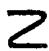
\includegraphics[keepaspectratio]{images/part001_579990b7.jpg}}

设 (C, d) 为一个复形。我们令 \(\mathbf{Z}(\mathbf{C}, d) = \operatorname{Ker}(d)\) , \(\mathbf{B}(\mathbf{C}, d) = \operatorname{Im}(d)\) ，它们是 C 的分次子模，分别称为 (C, d) 的闭链模和边缘模；\(\mathbf{Z}(\mathbf{C}, d)\) 和 \(\mathbf{B}(\mathbf{C}, d)\) 的齐次分量被记为 \(\mathbf{Z}_{n}(\mathbf{C}, d) = \mathbf{Z}^{-n}(\mathbf{C}, d)\) , \(\mathbf{B}_{n}(\mathbf{C}, d) = \mathbf{B}^{-n}(\mathbf{C}, d)\) ；我们有 \(\mathbf{Z}_{n}(\mathbf{C}, d) = \operatorname{Ker}(d_{n})\) , \(\mathbf{B}_{n}(\mathbf{C}, d) = \operatorname{Im}(d_{n+1})\) , \(\mathbf{Z}^{n}(\mathbf{C}, d) = \operatorname{Ker}(d^{n})\) , \(\mathbf{B}^{n}(\mathbf{C}, d) = \operatorname{Im}(d^{n-1})\) .

由于 \(d \circ d = 0\) ，我们有 \(\mathrm{B}(\mathrm{C}) \subset \mathrm{Z}(\mathrm{C})\) ；两个闭链若其差为一个边缘，则称它们是同调的；商分次模 \(\mathrm{H}(\mathrm{C}, d) = \mathrm{Z}(\mathrm{C}, d)/\mathrm{B}(\mathrm{C}, d)\) 被称为 \((\mathrm{C}, d)\) 的同调模；其元素是同调类；其齐次分量记为 \(\mathrm{H}_n(\mathrm{C}, d) = \mathrm{H}^{-n}(\mathrm{C}, d)\) 。

例。--- 若 C 的微分为零，则有 \(Z(C) = C\) , \(B(C) = 0\) ，且 \(H(C)\) 典范地等同于 \(C\) 。

我们有正合序列，称为典范的：

\((I_{n})\)

\[
0 \longrightarrow \mathrm{Z} _ {n} (\mathrm{C}) \longrightarrow \mathrm{C} _ {n} \stackrel {\delta_ {n}} {\longrightarrow} \mathrm{B} _ {n - 1} (\mathrm{C}) \longrightarrow 0\tag{\((\mathrm{II}_{n})\)}
\]

\[
0 \longrightarrow \mathrm{B} _ {n} (\mathrm{C}) \longrightarrow \mathrm{Z} _ {n} (\mathrm{C}) \longrightarrow \mathrm{H} _ {n} (\mathrm{C}) \longrightarrow 0
\]

\((\mathrm{III}_{n})\)

\[
0 \longrightarrow \mathrm{B} _ {n} (\mathrm{C}) \longrightarrow \mathrm{C} _ {n} \longrightarrow \mathrm{C} _ {n} / \mathrm{B} _ {n} (\mathrm{C}) \longrightarrow 0
\]

\((\mathrm{IV}_n)\)

\[
0 \longrightarrow \mathrm{H} _ {n} (\mathrm{C}) \longrightarrow \mathrm{C} _ {n} / \mathrm{B} _ {n} (\mathrm{C}) \stackrel {\overline {{\delta}} _ {n}} {\longrightarrow} \mathrm{B} _ {n - 1} (\mathrm{C}) \longrightarrow 0
\]

其中 \(\delta_{n}\) 和 \(\overline{\delta}_{n}\) 由 \(d_{n}\) 推出。通过结合 \((\mathrm{IV}_{n})\) 和 \((\mathrm{II}_{n-1})\) ，得到正合序列

\[
0 \rightarrow \mathrm{H} _ {n} (\mathrm{C}) \rightarrow \mathrm{C} _ {n} / \mathrm{B} _ {n} (\mathrm{C}) \rightarrow \mathrm{Z} _ {n - 1} (\mathrm{C}) \rightarrow \mathrm{H} _ {n - 1} (\mathrm{C}) \rightarrow 0,\tag{\((\mathbf{V}_n)\)}
\]

将 n 换成 -n，也可将它写成

\[
0 \rightarrow \mathrm{H} ^ {n} (\mathrm{C}) \rightarrow \mathrm{C} ^ {n} / \mathrm{B} ^ {n} (\mathrm{C}) \rightarrow \mathrm{Z} ^ {n + 1} (\mathrm{C}) \rightarrow , \mathrm{H} ^ {n + 1} (\mathrm{C}) \rightarrow 0.\tag{\((\mathbf{V}^n)\)}
\]

定义2.——设(C, d)和(C', d')是两个复形。从 (C, d) 到 (C', d') 的态射 \(^{1}\) 是从 C 到 C' 的次数为 0 的分次 A-同态 u，使得

\[
d ^ {\prime} \circ u = u \circ d.
\]

对于每一个 \(n\) ，我们有 \(d_n' \circ u_n = u_{n-1} \circ d_n\) 和 \(d''n \circ u^n = u^{n+1} \circ d^n\) 。我们有

\[
u (\mathbf {Z} (\mathbf {C})) \subset \mathbf {Z} (\mathbf {C} ^ {\prime}), \quad u (\mathbf {B} (\mathbf {C})) \subset \mathbf {B} (\mathbf {C} ^ {\prime}),
\]

并且我们用 \(Z(u):Z(C)\to Z(C')\) , \(B(u):B(C)\to B(C')\) , \(H(u):H(C)\to H(C')\) 表示由它们推出的A-模同态；这些态射的齐次分量记为 \(Z_{n}(u)\) , \(Z^{n}(u)\) , \ldots{}

若 \(v\) 是另一个从 \((\mathbf{C}, d)\) 到 \((\mathbf{C}', d')\) 的态射，则 \(u + v\) 是从 \((\mathbf{C}, d)\) 到 \((\mathbf{C}', d')\) 的态射，并且我们有

\[
\mathbf {Z} (u + v) = \mathbf {Z} (u) + \mathbf {Z} (v), \quad \mathbf {B} (u + v) = \mathbf {B} (u) + \mathbf {B} (v), \quad \mathbf {H} (u + v) = \mathbf {H} (u) + \mathbf {H} (v)
\]

类似地，若A是交换环 \(k\) 上的代数，且如果 \(\lambda \in k\) ，则 \(\lambda u\) 是从 \((C, d)\) 到 \((C', d')\) 的态射，并且我们有

\[
\mathbf {Z} (\lambda u) = \lambda \mathbf {Z} (u), \quad \mathbf {B} (\lambda u) = \lambda \mathbf {B} (u), \quad \mathbf {H} (\lambda u) = \lambda \mathbf {H} (u).
\]

若 \(u': (C', d') \to (C'', d'')\) 是另一个复形态射，则 \(u' \circ u\) 是从 \((C, d)\) 到 \((C'', d'')\) 的态射，并且我们有

\[
\mathrm{Z} \left(u ^ {\prime} \circ u\right) = \mathrm{Z} \left(u ^ {\prime}\right) \circ \mathrm{Z} (u), \quad \mathrm{B} \left(u ^ {\prime} \circ u\right) = \mathrm{B} \left(u ^ {\prime}\right) \circ \mathrm{B} (u), \quad \mathrm{H} \left(u ^ {\prime} \circ u\right) = \mathrm{H} \left(u ^ {\prime}\right) \circ \mathrm{H} (u).
\]

显然，双射态射即同构。

定义3.——设(C, d)和(C', d')是两个复形。从(C, d)到(C', d')的同调态射（或拟同构）是一个从(C, d)到(C', d')的态射u，使得H(u)是双射。

每个同构都是同调态射，并且由同调态射复合而成的任何态射都是同调态射。

称(C, d)具有零同调，若H(C) = 0，即若唯一的复形态射 \(0 \rightarrow C\) （相应地，C → 0）是一个同调态射。称（C, d）在降次数 n（相应地，在升次数 n）上是零调的，如果 \(\mathrm{H}_{n}(\mathrm{C}) = 0\) (相应地， \(\mathrm{H}^{n}(\mathrm{C}) = 0\) ).

设 (C, d) 为一个复形且 \(p \in Z\) ；(C, d) 的第 p 次平移是如下得到的复形 (C(p), d(p))：C(p) 是通过将 C 的分次平移 p 得到的 A-模（II，第 163 页；例 3），因此

\[
\mathrm{C} (p) _ {n} = \mathrm{C} _ {n + p}, \quad \mathrm{C} (p) ^ {n} = \mathrm{C} ^ {n - p};
\]

特别地 \(\mathbf{C}(p)_{0} = \mathbf{C}_{p}\) ；还需注意 C 是其分次子模 \(\mathbf{C}_{p}(-p)\) , \(p \in \mathbf{Z}\) （相应地， \(\mathbf{C}^{p}(p)\) , \(p \in \mathbf{Z}\) ）的直和。定义 \(d(p) = (-1)^{p} d\) 。我们有 \(\mathbf{Z}(\mathbf{C}(p)) = \mathbf{Z}(\mathbf{C})(p)\) , \(\mathbf{B}(\mathbf{C}(p)) = \mathbf{B}(\mathbf{C})(p)\) 和 \(\mathrm{H}(\mathbf{C}(p)) = \mathrm{H}(\mathbf{C})(p)\) 。

例如， \(d\) 是从 C 到 C(-1) 的复形态射，并且

\[
\mathrm{H} (d): \mathrm{H} (\mathbf {C}) \to \mathrm{H} (\mathbf {C}) (- 1)
\]

是零。

对于每个复形态射 \(u:(\mathbf{C},d)\to(\mathbf{C}^{\prime},d^{\prime})\) ，以及每个 \(p\in\mathbf{Z}\) , \(u\) 也是从 \((\mathbf{C}(p),d(p))\) 到 \((\mathbf{C}^{\prime}(p),d^{\prime}(p))\) 的态射；它有时被记为 \(u(p)\) 并且我们有

\[
u (p) _ {n} = u _ {n + p}, \quad u (p) ^ {n} = u ^ {n - p}.
\]
